\documentclass[letterpaper,oneside,12pt]{report}

\usepackage{amsmath,amssymb,amsfonts,latexsym,cancel} %Soporte para math
\usepackage[pdftex]{graphicx}			%Soporte para gráficos..
\usepackage[pdftex,margin=1in]{geometry}			%to make letterpaper work

\usepackage{float}		% to show floating figures
\usepackage{listings}	% to add source codes
\usepackage{color}		% colored fonts

\DeclareGraphicsExtensions{.pdf,.png,.jpg}
\DeclareGraphicsRule{.wmf}{bmp}{}{}

\usepackage[utf8]{inputenc}			% Use for Linux (latin1 instead of utf8 for MS)
\usepackage[spanish]{babel}  		% Use this to change titles to Spanish
\usepackage{verbatim} 				% To allow \begin{comment}

% If the installation of the APACITE package is required,
% go to the latex folder and remove all the apacite*.* files
% _except_ for apacite.dtx and apacite.ins. Then run "latex apacite.ins"
% and it will install the required files.
\usepackage{apacite}
	
\usepackage{setspace}	% to set line spacing 


\begin{document}

\onehalfspace

\newcommand{\one}[1]{\mathbf{1}_{#1}}

\renewcommand{\contentsname}{Contenido}
\renewcommand{\partname}{Parte}
\renewcommand{\indexname}{Lista Alfabética}
\renewcommand{\appendixname}{Anexo}
\renewcommand{\figurename}{Figura}
\renewcommand{\listfigurename}{Lista de Figuras}
\renewcommand{\tablename}{Tabla}
\renewcommand{\listtablename}{Lista de Tablas}
\renewcommand{\abstractname}{Abstract}
\renewcommand{\chaptername}{Capítulo}
\renewcommand{\refname}{Referencias}


% Reset some commands to the default, to change the biography display:
% http://www.cs.ucf.edu/~leavens/texmf/tex/latex/misc/apacite.sty
\renewcommand{\BOthers}[1]{et al.{}}
\renewcommand{\BOthersPeriod}[1]{et al.{}}


% list options
\renewcommand{\labelitemi}{$-$}
\renewcommand{\labelitemii}{$\cdot$}
\renewcommand{\labelitemiii}{$\circ$}
\renewcommand{\labelitemiv}{$\bullet$}

\renewcommand{\@listI}{%
\leftmargin=50pt
\rightmargin=0pt
\labelsep=5pt
\labelwidth=20pt
\itemindent=0pt
\listparindent=0pt
\topsep=0pt plus 2pt minus 4pt
\partopsep=0pt plus 1pt minus 1pt
\parsep=-5pt
\itemsep=\parsep}




\begin{titlepage}

\begin{center}

\includegraphics[scale=0.30]{uade-logo.jpg}

\textsc{\Large UNIVERSIDAD ARGENTINA DE LA EMPRESA}\\[0.5cm]

\vspace*{0.5cm}
\textsc{\Large Departamento de Economía y Finanzas}\\[0.5cm]

\vspace*{2cm}

% Title
%\rule{\linewidth}{0.5mm} \\[0.4cm]
{ \huge \bfseries Utilización del CAPM para la \\
		Valuación de Opciones}\\[0.4cm]

\vspace*{0.5cm}

\textsc{\large Trabajo de Investigación Final en Finanzas}\\[0.5cm]


%\rule{\linewidth}{0.5mm} \\[1.5cm]


\large{\emph{Tutor:} Dr. Marcelo \textsc{Perillo}}

\vfill

% Bottom of the page

\emph{Autor:} Diego \textsc{Jancic}

\vspace*{2cm}

{\large \today}

\end{center}

\end{titlepage}


\begin{center}
	\bf Abstract
\end{center}

This essay presents the development of the capital asset pricing model (CAPM) as a method for pricing stock options. It begins with a review of the traditional method of the valuation of assets under market equilibrium.  Then the main methods for pricing options are presented, which are the Black-Merton-Scholes and the binomial tree. Finally the mathematical equivalency of these models is verified and then the results are analyzed by using a computer simulation.

The ultimate goal is to show the valuation capacity of the CAPM and its correlation with the traditional methods for pricing options.

\vspace{1.5cm}
\begin{center}
	\bf Resumen
\end{center}

En el presente trabajo se desarrolla al modelo de valuación de activos de capital (CAPM) como método para la valuación de opciones. Primero se hace un repaso del método clasico de valuación de activos bajo la situación de equilibrio de mercado. Luego se presentan los principales métodos de valuación de opciones, siendo estos el modelo de Black-Merton-Scholes y el de arboles binomiales. Por último se verifica la equivalencia matemática de dichos modelos y se analiza el comportamiento de estos con la utilización de una simulación.

El objetivo final es mostrar la capacidad de valuación del mencionado \textit{Capital Asset Pricing Model}, y su correlato con los métodos tradicionales de valuación de opciones.

\thispagestyle{empty}

\setcounter{page}{1}
\include{Indice}


\chapter*{Introducción}\label{introduccion}
\addcontentsline{toc}{chapter}{Introducción}

En el presente trabajo se aborda la problemática de la valuación de un tipo de instrumento financiero que se negocia en gran volumen en los mercados de capitales del mundo. Éstos, conocidos como opciones sobre acciones de tipo europeo, son contratos a través de los cuales el inversor tiene el derecho, pero no la obligación, de comprar o vender la acción subyacente en una determinada fecha \cite{hull}. Cuando un participante de mercado desea asignarle un precio a estos activos, puede recurrir a alguno de los modelos financieros de valuación que proporcionan las finanzas.

Entre ellos podemos mencionar el Modelo de Valuación de Activos de Capital (CAPM, por sus siglas en inglés), siendo este el más utilizado tanto en el ámbito profesional como en el académico debido a la simpleza de los supuestos económicos en los que se basa. Dada la amplitud de este modelo, el mismo es conceptualmente utilizable para valuar cualquier tipo de instrumento financiero, incluso las opciones de tipo europeo cuyo análisis es el objetivo del presente trabajo. Sin embargo, si bien el CAPM es uno de los métodos con mayor aceptación para la valuación de diversos activos, es poco frecuente su utilización en estos contratos.

En 1973, Fisher Black y Myron Scholes (B\&S) desarrollaron otro modelo para valuar opciones europeas, el cual se conoce por el nombre de sus creadores. Entre los profesionales del área, este modelo fue pionero para la valuación de dichos instrumentos, y desde entonces ha sido el de mayor difusión debido a que su aplicación es matemáticamente simple. Esta ecuación, que le valió el premio Nobel a Myron Scholes, es ampliamente utilizada en la actualidad por los participantes del mercado de opciones.

El objetivo general de este trabajo es comprobar que la valuación de una opción europea mediante CAPM es posible, y que su utilización conduce a los mismos resultados que el modelo desarrollado por B\&S. En teoría, es esperable que los dos modelos mencionados sean válidos y que su utilización no conlleve a resultados contrapuestos.

A su vez, se mostrará que el riesgo de esta clase de instrumentos medido por su \textit{beta} ($\beta$) es considerablemente mayor al de las acciones asociadas. De la misma forma, se espera verificar que la medida de riesgo $ \beta $ de éstos varía continuamente con el paso del tiempo, a diferencia de la de los activos subyacentes, que se asume constante.

La comparación se realizará entre dos modelos teóricos para la valuación de opciones. A efectos de analizar la precisión de los resultados de dichos modelos, es necesario utilizar valores numéricos como \textit{input}. Si bien los datos pueden obtenerse del mercado, esto no aportaría valor al análisis ya que la existencia en la realidad de dichos valores no es de importancia. Específicamente, será necesario conocer datos como el precio de una acción, su volatilidad y el tiempo al vencimiento de la opción; todos ellos son valores que no se encuentran relacionados entre sí, y por ende pueden utilizarse valores ficticios a la hora de comprobar la viabilidad práctica del modelo. 

No se partirá de ninguna fuente de datos para comprobar los modelos, serán simplemente supuestos que sirvan para continuar con el desarrollo de los ejemplos presentados. Una vez que se obtengan los resultados de los modelos bajo estudio, las comparaciones y el análisis requerido se hará sobre estos resultados.

Dada el metodología utilizada, los resultados del análisis serán atemporales y aplicables a cualquier mercado que cumpla, al menos, con los supuestos en los que se base cada modelo (véase secciones 1.1 y 2.3).



\section*{¿Qué son las opciones?}
\addcontentsline{toc}{section}{¿Qué son las opciones?}

Se conoce con este nombre a un tipo de contrato que se realiza exclusivamente entre dos partes, la emisora y la compradora del mismo. La primera, se obliga a comprar o vender un activo subyacente a un determinado precio si el adquirente del contrato lo desea. Desde la óptica del comprador del contrato, es un derecho a realizar la compra o venta de un determinado activo, en un momento o en un plazo de tiempo prefijado en el contrato \cite{hull}.

Es necesario definir algunos términos para comprender esto. Primero, se denomina activo subyacente a un valor negociable, el cual es sujeto de intercambio en caso de ejercerse la opción. Por ejemplo, son activos subyacentes las acciones de empresas, los contratos de futuros sobre \textit{commodities} y los títulos de renta fija, entre otros. Así mismo, el contrato define el precio al cual se efectuará la operación de compra o venta, o \textit{Strike Price}. La fecha de ejercicio es otro factor importante, ya que define el periodo de validez del contrato; una vez pasada esa fecha, si el derecho no se ejerció, el contrato queda sin efecto.

Estos contratos son negociados activamente en la actualidad, siendo un mercado que tiene menos de treinta años, solo en la bolsa de comercio de opciones de Chicago se negocian más de mil millones de contratos al año \cite{cboe}. Eso es muestra de la importancia que cobran estos activos en los mercados de valores en la actualidad.

Al ser un contrato, éste puede tomar una incontable cantidad de formas. Incluso existen opciones exóticas o no estándar negociadas en mercados no regulados. Pero es preciso describir las que se negocian con mayor volumen en los mercados abiertos.

El primer aspecto relevante es que una opción puede ser de compra (\textit{call}) o de venta (\textit{put}). Las primeras dan el derecho al adquirente de la misma a comprar el activo subyacente al \textit{Strike Price} prefijado. Por el contrario, las \textit{put}, dan el derecho de venta del subyacente. El activo sobre el cual subyace la opción puede ser una acción, un índice bursátil o el estado de un crédito, entre otros \cite{elton}. De las características de este activo dependerá en gran medida el valor de la opción negociada.

Otra característica importante tiene que ver con el periodo en el cual se puede ejercer la opción. En base a esto, se dividen en opciones europeas y americanas; clasificación que no está relacionada con la ubicación geográfica de la misma \cite{hull}. Las opciones americanas son ejercibles durante todo el periodo de validez del contrato, mientras que las europeas sólo lo son a la finalización del contrato. A modo de ejemplo, si una opción americana \textit{call} con fecha de vencimiento en mayo es comprada en enero, el inversor puede ejercerla en cualquier momento entre enero y mayo. Si, en cambio, la opción fuese europea, solo podría ejercerla el día que vence (en mayo).

Si bien existe una amplia gama de opciones como se explicó anteriormente, en el presente trabajo se analiza la valuación de opciones europeas sobre acciones que no pagan dividendos, ya sean del tipo \textit{call} o \textit{put}. La restricción en el análisis se debe a que estas pueden ser valuadas mediante los dos modelos que se desarrollan, el CAPM y el de B\&S.

El monto que paga una opción del tipo \textit{call} si se ejerce al vencimiento, conocido como \textit{payoff}, es igual al precio del subyacente en ese momento menos el precio de ejercicio. En caso de que esto último sea negativo, un inversor racional optaría por no ejercer su derecho y por lo tanto el mismo expiraría sin obtener ningún resultado. En ambos casos, el comprador realizó una inversión inicial para adquirir el derecho, por lo que esto debe restarse para obtener el resultado neto de la operación. En el caso de opciones \textit{put}, el razonamiento es inverso: la ganancia será el precio de ejercicio menos el valor del subyacente en el momento que se ejerce, o cero en el caso en que este resultado sea negativo. Estos resultados serán analizados en más detalle en los siguientes capítulos.



\chapter{Capital Asset Pricing Model}\label{CAPM}

\section{Principios básicos}

Se conoce con el nombre de Modelo de Valuación de Activos de Capital (CAPM, por sus siglas en inglés), a la teoría desarrollada principalmente por William Sharp en 1964 en base a trabajos previos de Harry Markowitz y James Tobin \cite{sharp}. Mediante este modelo se puede determinar la relación entre la rentabilidad de un activo cualquiera y su riesgo asociado, por lo que es de gran utilidad en la teoría de administración de portafolios de inversión. 

Un portafolio perfectamente diversificado, que contenga todos los activos existentes en el mercado, no es afectado por las variaciones particulares que pueda sufrir un activo\footnote{Para una comprobación rigurosa, véase Elton y Gruber (1995).\nocite{elton}}. Esto se debe a que el riesgo individual de cada activo es muy pequeño en comparación con la cartera, por lo que lo único que es relevante en este caso es el riesgo sistémico\footnote{Riesgo sistémico es aquel que afecta a todo el mercado, como puede ser una noticia de orden macroeconómico.}. Ahora, si consideramos al mercado como base de análisis, cada activo tendrá una sensibilidad mayor o menor a las variaciones de la economía.

Lo enunciado en el párrafo anterior es una explicación conceptual del CAPM. Considerando el razonamiento de un inversor racional y averso al riesgo, para realizar una inversión que tenga riesgos asociados, siempre se esperará que el rendimiento sea mayor a la tasa pagadera por un activo libre de riesgo.

Este modelo presenta una forma de equilibrio general que permite ver la relación entre riesgo y rentabilidad de los activos \cite{elton}. La ventaja de esta relación es que hace al CAPM capaz de valuar cualquier tipo de activo en el mercado. Se considera un mundo ideal con el objetivo de agregar simplicidad al modelo, lo que implica tomar en cuenta una serie de supuestos \cite{elton}.

Primero, se asume la ausencia de costos de transacción, ya que de otra forma habría que considerar el hecho de si el inversor ya poseía activos en su cartera, o los adquirió posteriormente. 

Segundo, los activos se consideran infinitamente divisibles, esto es esencial ya que un portafolio bien diversificado (como uno equivalente a todo el mercado) debe contener una parte pequeña de cada activo. 

En tercer lugar se asume la inexistencia de efectos fiscales como el impuesto a las ganancias, de esta forma se eliminan todas las distorsiones que estos puedan provocar. 

Cuarto, un solo inversor no puede afectar el precio de un activo, ya que esto provocaría variaciones en los precios de los activos por el solo hecho de adquirirlos, lo que desvirtuaría el análisis completamente. 

El quinto supuesto esta relacionado con la forma en la que los inversores toman sus decisiones. Debido a que el CAPM utiliza como base un portafolio equivalente al mercado, es necesario que este sea eficiente y que los otros agentes de mercado armen su cartera racionalmente maximizando el rendimiento para un nivel de riesgo.

En sexto lugar, los inversores pueden realizar de manera ilimitada ventas en corto (\textit{short sales}), así como pueden colocar y pedir prestado a la tasa de interés libre de riesgo.

Por último, se considera que todos los agentes de mercado disponen de la misma información y por lo tanto hay homogeneidad de expectativas. A su vez, es necesario remarcar que los activos deben ser comerciables, aspecto que no necesariamente se cumple en mercados no desarrollados por razones de iliquidez.


\section{El problema del inversor}

\subsection{La utilidad obtenida}

Tomando el supuesto de que una persona cualquiera toma sus decisiones de inversión en base a la rentabilidad y el riesgo esperado \cite{sharp}, es posible analizar como será su selección de activos.

Existen dos formas funcionales esenciales para analizar la selección de activos. Primero, la función de utilidad de un inversor que puede expresarse en términos de rentabilidad esperada \cite{sharp}:

\begin{align}
	U = U(\overline{r_i} ; \sigma_i) \label{funcionutilidad}
\end{align}

Donde $\overline{r_i}$ es la rentabilidad esperada de la inversión y $\sigma_i$ es el riesgo, medido como el desvío entre la rentabilidad esperada y la posiblemente obtenida. $U$ en función del rendimiento será positivo ($\partial U/\partial r_i > 0$) debido a que un inversor obtendrá lógicamente mayor utilidad a medida que la rendimiento aumenta, manteniendo el riesgo constante. Inversamente, $U$ en función del riesgo será negativo ($\partial U/\partial \sigma_i < 0$), \textit{ceteris paribus}.

\begin{figure}[H]
\centering
\includegraphics[width=1\textwidth]{Images/capm.png}
\caption{Frontera de eficiencia, \textit{CAL} y curvas de isoutilidad}
\label{fig:frontef}
\end{figure}

La figura \ref{fig:frontef} muestra las curvas de isoutilidad, es decir que todos los punto sobre cada una de ellas representan la misma utilidad para el inversor. La elección entre dos portafolios ubicados sobre la misma curva de isoutilidad le es indistinta al inversor. Cuanto más arriba se encuentre la curva, mayor utilidad total presentará debido a que de dos portafolios con el mismo riesgo siempre es preferible aquel que se espera tenga mayor rendimiento. De la misma forma, de dos portafolios con el mismo rendimiento esperado, siempre es preferible el que tenga menor riesgo.

Resolver el problema del inversor consistirá en encontrar el portafolio que maximice la utilidad del inversor, sujeto a la limitación de los posibles portafolios construibles.

\subsection{Selección de portafolio}

La segunda función a analizar es la de la frontera de portafolios posibles. Si un inversor decide distribuir el total de su capital en dos o más activos de riesgo, de acuerdo a como distribuya su capital, podrá obtener distintos portafolios resultantes. En el caso en que dichos activos no se encuentren perfectamente correlacionados, la función resultante de opciones posibles será una curva convexa que se encuentre por sobre todos los activos considerados. Esta curva, o frontera de eficiencia, se encuentra representada en la figura \ref{fig:frontef}.

La forma de la frontera de eficiencia se debe a que la correlación no es perfecta entre todos los activos \cite[p.430]{sharp}. Esto es demostrable fácilmente si se calcula el desvío esperado de una combinación de dos activos riesgosos, ya que la tanto el rendimiento como el desvío dependerán de las proporciones invertidas en cada activo, este último de forma no lineal. Por ejemplo, si se deposita $\alpha$ en el activo 1 y $(1-\alpha)$ en el activo 2, el retorno y el desvío del portafolio resultante serán: 

\begin{align}
	\overline{r_P} &= \alpha \overline{r_1} + (1-\alpha) \overline{r_2} \label{renddosactivos} \\
	\sigma_P &= \left[ \alpha^2 \sigma_1^2 + (1-\alpha)^2 \sigma_2^2 + 
		2 \alpha (1-\alpha) \sigma_{12} \right]^{1/2} \label{desviodosactivos}
\end{align}

Donde $\overline{r_P}$ y $\sigma_P$ son el rendimiento esperado y el desvío de los rendimientos del portafolio, $\overline{r_i}$ y $\sigma_i$ son el rendimiento esperado y el desvío de los rendimientos del activo $i$, y $\alpha$ es la proporción invertida en el activo 1.

Una vez construida la frontera de eficiencia, producto de la combinación de activos riesgosos, se debe seleccionar el portafolio adecuado. Si se toma como supuesto que el inversor puede colocar y tomar prestado a la tasa libre de riesgo ($r_f$), el portafolio final resultante ($P$) será entonces una combinación lineal entre esta y el portafolio riesgoso ($Z$). Por ende, $P$ será el resultado de la combinación entre $Z$ y $r_f$, siendo este último un activo sin riesgo y por ende no correlacionado con $Z$.

Las diferentes combinaciones entre $Z$ y $r_f$ crean el conjunto de portafolios posibles. Cuando todos los portafolios combinación de estos se encuentran  sobre todo el conjunto abarcado por la frontera de eficiencia, entonces la recta que surge de unir estos dos puntos maximiza la elección del inversor.. A esta recta se la conoce como \textit{Capital Allocation Line} (\textit{CAL}) y se encuentra representada en la figura \ref{fig:frontef}. La \textit{CAL} es entonces la recta de mayor pendiente, que maximiza a su vez la utilidad del inversor.

Extendiendo las ecuaciones \eqref{renddosactivos} y \eqref{desviodosactivos} al caso de $n$ activos, el rendimiento esperado del portafolio se calculará como el promedio ponderado de los activos que lo componen. En el caso del riesgo del portafolio, o desvío estándar de los rendimientos, este se calcula como muestra la ecuación \eqref{varportafolio}.

\begin{align}
	\overline{r_P} &= w_1 \overline{r_1} + w_2 \overline{r_2} + \dotsb + 
		w_n \overline{r_n} = \sum\limits_{i=1}^n w_i \overline{r_i} \label{rendportafolio} \\
	\sigma_P^2 &= \sum\limits_{i=1}^n w_i^2 \overline{r_i}^2 + 
		\sum\limits_{i=1}^n \sum\limits_{\substack{j=1 \\ i \neq j}}^n w_i w_j \sigma_{ij}  \label{varportafolio}
\end{align}

Donde $w_i$ es la proporción del activo $i$ en la cartera. A continuación se deriva la fórmula de la pendiente de la \textit{CAL} para el caso de $n$ activos.


\section{Portafolio óptimo}

Como puede apreciarse en la figura \ref{fig:frontef}, la pendiente de la \textit{CAL} ($\theta$) puede ser expresada de la siguiente forma:

\begin{align}
	\theta = \frac{\overline{r_P} - r_f}{\sigma_P}
\end{align} 

Para obtener el conjunto de portafolios eficientes es necesario encontrar la recta que posea mayor pendiente. Esto se debe a que al maximizarla, sea cuales sean las curvas de isoutilidad del inversor, la máxima utilidad se obtendrá en la intersección con la \textit{CAL}.

Entonces, maximizando la pendiente:

\begin{align}
	\mbox{max } \theta = \frac{\overline{r_P} - r_f}{\sigma_P} \label{maxptecal}
\end{align}

Con respecto a $w_i$ y sujeto a:

\begin{align}
\mbox{Restricciones} \left\{  \nonumber
	\begin{array}{l}
		\mbox{1) } \overline{r_P} = w_1 \overline{r_1} + w_2 \overline{r_2} + \dotsb + 
			w_n \overline{r_n} = \sum\limits_{i=1}^n w_i \overline{r_i} \nonumber\\
		\mbox{2) } \sigma_P^2 = \sum\limits_{i=1}^n w_i^2 \overline{r_i}^2 + 
			\sum\limits_{i=1}^n \sum\limits_{\substack{j=1 \\ i \neq j}}^n w_i w_j \sigma_{ij}  \nonumber \\
		\mbox{3) } \sum\limits_{i=1}^n w_i = 1
	\end{array} \right.
\end{align}

La primer y tercer restricción pueden ser reemplazadas en la fórmula de la pendiente de la CAL. Debido a que $\sum w_i r_f = r_f$, se obtiene que $\theta$ estará dado por:

\begin{align}
	\theta = \left[ \sum\limits_{i=1}^n w_i (\overline{r_i} - r_f) \right] 
		\left( \sum\limits_{i=1}^n w_i^2 \overline{r_i}^2 + \sum\limits_{i=1}^n 
		\sum\limits_{\substack{j=1 \\ i \neq j}}^n w_i w_j \sigma_{ij} \right)^{-1/2}
\end{align}

Ahora, derivando $\theta$ en función de cada proporción en la cartera $w_i$ e igualando a cero, es posible obtener el máximo de la función. Esto quiere decir que el resultado que maximice la pendiente de la CAL será aquel que haga cero todas las derivadas parciales de la misma. Formalmente:

\begin{align}
	\frac{\partial \theta}{\partial w_i} = 0 \quad \forall \quad 1 \leq i \leq n
\end{align}

Entonces, igualando la derivada a cero y despejando se llega a lo siguiente:

\begin{align}
	\overline{r_i} - r_f = \frac{\sum\limits_{i=1}^n w_i (\overline{r_i} - r_f)}{\sigma^2} 
		\left( w_i \sigma_i^2 + \sum\limits_{\substack{j=1 \\ j \neq i}}^n w_j \sigma_{ij} \right) \label{eqzetas1}
\end{align}

El primer término de la ecuación \eqref{eqzetas1} es igual a la rentabilidad en exceso del portafolio divido su desvío: $ (\overline{r_P} - r_f)/\sigma_P^2$. Para simplificar se puede llamar $Z_i$ a esto último multiplicado por la proporción de cada activo en el portafolio ($w_i$):

\begin{align}
	Z_i = \frac{\overline{r_P} - r_f}{\sigma_P^2} * w_i \label{formulazeta}
\end{align}

De esta forma obtenemos un conjunto de ecuaciones, una por cada derivada parcial de la ecuación \eqref{maxptecal} o, lo que es lo mismo, una por cada activo en el portafolio del inversor.

\begin{align}
	\left\{
	\begin{array}{l l}
		\overline{r_1} - r_f &= Z_1 \sigma_1^2 + Z_2 \sigma_{1 2} + \dotsb + Z_n \sigma_{1 n} \\
		\overline{r_2} - r_f &= Z_1 \sigma_{2 1} + Z_2 \sigma_2^2 + \dotsb + Z_n \sigma_{2 n} \\
		& \mbox{ }\vdots \\
		\overline{r_n} - r_f &= Z_1 \sigma_{n 1} + Z_2 \sigma_{n 2} + \dotsb + Z_n \sigma_n^2 
	\end{array} \right. \label{eczetas}
\end{align}


El sistema de ecuaciones \eqref{eczetas} resuelve la combinación óptima de activos según la teoría desarrollada por Markowitz. Este sistema puede ser fácilmente resuelto usando un sistema de matrices para averiguar los valores de $Z_i$. Luego, las proporciones pueden ser obtenidas haciendo $w_1 = \frac{Z_1}{\sum Z_i}$, $w_2 = \frac{Z_2}{\sum Z_i}$, ..., $w_n = \frac{Z_n}{\sum Z_i}$.

Con este método un inversor racional armaría su portafolio, lo que nos permite llevar este modelo aún más lejos y analizar el caso en donde todos los inversores optimizarían su portafolio de la misma forma. Esto si bien es hipotético dada la naturaleza de la afirmación, puede ser tomado como un supuesto válido para el modelo presentado a continuación.

\section{Derivación del CAPM}

Como se mencionó anteriormente, la teoría desarrollada por Harry Markowitz es la base de este modelo. Dicha teoría postula una forma eficiente de combinar activos cuando se forma una cartera de inversión, de forma de maximizar el rendimiento esperado dado un nivel de riesgo.

Si en el mercado existen una gran cantidad de activos riesgosos, la combinación de estos en diferentes cantidades pueden producir una infinita variedad de resultados. Sin embargo, en caso de existir dos activos con el mismo nivel de riesgo y diferente rentabilidad, un inversor racional sólo compraría el que tenga mayor rentabilidad. Más aún, lo lógico sería vender el activo que se espera que tenga un rendimiento menor  y con el dinero obtenido comprar de mayor ganancia esperada. Dado que en los dos activos el riesgo es igual, la ganancia en promedio será positiva. Esta clase de operaciones tendería a incrementar el precio de las acciones con mayor rendimiento esperado y a reducir el precio del resto. La dinámica generada por la oferta y la demanda de activos, crea una situación de equilibrio en donde todos los activos con igual riesgo poseen igual rendimiento esperado \cite{sharp}.

El inversor analizado en la sección anterior puede decidir diversificar su portafolio en una gran cantidad de activos, idealmente infinitos, para diluir el riesgo particular de cada activo \cite{effectofdiversification}. Si las proporciones de su portafolio se vuelven iguales a las proporciones de los activos en el mercado, se puede decir que su portafolio es igual al del mercado (en términos de $w_i$). Para el caso bajo análisis la fórmula \eqref{formulazeta} queda:

\begin{align}
	Z_i = \frac{\overline{r_M} - r_f}{\sigma_M^2} * w_i \label{formulazetamercado}
\end{align}

Nótese que la única diferencia entre \eqref{formulazeta} y \eqref{formulazetamercado} es que la segunda considera el rendimiento esperado del mercado (notado $\overline{r_M}$) y la varianza del mismo, las cuales son iguales a las del portafolio. Ahora, tomando un activo cualquiera, la ecuación del portafolio óptimo \eqref{eqzetas1} queda:

\begin{align}
	\overline{r_i} - r_f = \frac{\overline{r_M} - r_f}{\sigma_M^2} 
		\underbrace{\left( \sum\limits_{j=1}^n w_j \sigma_{ij} \right)}_{Cov(r_i; r_M)}
\end{align}

Debido a que el segundo término es igual a la covarianza entre los rendimientos de $i$ y los del mercado
\footnote{Demostración: \begin{align}
		Cov(r_i, r_M) &= E[(r_i-\overline{r_i})(r_M-\overline{r_M})] \nonumber\\
			&= E[(r_i-\overline{r_i})(\sum\limits_{j=1}^n w_j r_j-\sum\limits_{j=1}^n w_j \overline{r_j})] \nonumber\\
			&= \sum\limits_{j=1}^n w_j E[(r_i-\overline{r_i})(r_j-\overline{r_j})]
			= \sum\limits_{j=1}^n w_i \sigma_{ij} \nonumber
		\end{align}}, se puede despejar la rentabilidad del activo:

\begin{align}
	\overline{r_i} = r_f + \frac{Cov(r_i; r_M)}{\sigma_M^2} ( \overline{r_M} - r_f )
\end{align}

Finalmente, la expresión $ Cov(r_i; r_M) / \sigma_M^2$ puede ser reemplazada con la letra griega $\beta$. \textit{CAPM} se expresa normalmente de la siguiente forma:

\begin{align}
	\overline{r_i} = r_f + \beta ( \overline{r_M} - r_f ) \label{capm}
\end{align}

La letra \textit{beta} representa la relacion de rentabilidad y riesgo histórico entre un activo y un portafolio igual al mercado. El hecho de que sea una relación histórica se debe a que normalmente el \textit{beta} se obtiene mediante una regresión lineal de los valores del mercado. Esto no niega que el \textit{CAPM} sea adecuado al mostrar la relación entre rentabilidad y riesgo, al menos en el largo plazo \cite[p.357]{elton}.


\section{Características de \textit{Beta}}

Como se explicó en la sección anterior, el \textit{beta} de un activo es igual a la covarianza del mismo contra el mercado, dividido la varianza del mercado. Si la varianza del mercado en un momento particular está dada, dos activos con distinta covarianza con el mercado tendrán diferente \textit{beta}. A mayor covarianza la $\beta$ será también mayor. 

Que un activo posea $\beta = 1$ significa que un cambio en el mercado provocará un cambio de igual magnitud en dicho activo, o al menos eso se espera. La razón de esto es que la \textit{beta} del mercado es por definición igual a uno, al ser la covarianza entre dos rendimientos iguales (mercado contra mercado) igual a la varianza ($\sigma_M^2 / \sigma_M^2 = 1$). Si el \textit{beta} es mayor que uno, un movimiento sistémico producirá un cambio aún mayor en el activo. Lo opuesto ocurrirá si $\beta < 1$.

Cuando un portafolio se encuentra altamente diversificado, los \textit{shocks} particulares de cada activo tienen a ser insignificantes y desaparecer en el portafolio \cite{sharp}. Es por esto que el impacto que sufre un activo en particular debido a \textit{shocks} sistémicos es el único relevante, siendo esto lo que el \textit{beta} mide.

El \textit{beta} de un portafolio puede ser calculado a partir del rendimiento esperado para un conjunto de $n$ activos, utilizando \textit{CAPM}:

\begin{align}
	\sum\limits_{i=1}^n w_i \overline{r_i} &= \sum\limits_{i=1}^n w_i \left[ r_f + 
		\beta_i (\overline{r_M} - \overline{r_f}) \right] \label{sumatoriacapm} \\
	\mbox{con } \sum\limits_{i=1}^n w_i &= 1 \nonumber
\end{align}

Como $\sum w_i \overline{r_i} = \overline{r_P}$, reorganizando la ecuación \eqref{sumatoriacapm} obtenemos:


\begin{align}
	\underbrace{\sum\limits_{i=1}^n w_i \overline{r_i}}_{r_P} &= r_f + 
		\underbrace{\sum\limits_{i=1}^n \beta_i}_{\beta_P} (\overline{r_M} - \overline{r_f}) \label{betaportafolio}
\end{align}


Por lo que el \textit{beta} de un conjunto de activos es igual al promedio de los $\beta$s ponderado por el peso que cada uno de estos tiene en la cartera. Siguiendo con este razonamiento, cuando $n$ es igual a la cantidad de activos del mercado, el \textit{beta} del mercado deberá ser igual a uno para que la ecuación \eqref{betaportafolio} sea válida.



















\chapter{Modelos de valuación de opciones}

\section{El nacimiento de nuevo mercado}

Desde 1973, los contratos de opciones son comerciados a diario en los mercados públicos, siendo el más importante en términos de volumen negociado el \textit{Chicago Board or Options Exchange} (2011)\nocite{cboe}; mercado en el que actualmente se negocian millones de contratos diariamente. Dicho año coincide con el desarrollo de un modelo matemático para la valuación de opciones, realizado por Fisher Black, Myron Scholes y Robert Merton. El desarrollo del mismo fue razón de importante crecimiento en el mercado de opciones, y fue de gran importancia para el desarrollo de la ingeniería financiera en los últimos años \cite{hull}.

El crecimiento de este mercado se dio en gran medida a causa del desarrollo de este método para valuar opciones. Actualmente sigue siendo utilizado en gran medida en el ámbito profesional y académico. De ahí, la importancia que tiene a la hora de valuar opciones.

En este capítulo se desarrolla los conceptos del modelo de Black-Scholes-Merton (o Black-Scholes) para la valuación de opciones europeas sobre acciones que no pagan dividendos.

\section{Características de las opciones}

El valor de una opción depende de varios factores. Debido a que estas pueden ser entendidas como seguros ante el alza o ante la baja en el precio del subyacente, se puede realizar un primer acercamiento a las variables involucradas. Al ser un seguro, cuanto mayor sea el riesgo de que este sea cobrado, mayor será la prima que se deberá pagar para adquirirlo.

En el caso de una opción de compra sobre una acción, por ejemplo, el valor de la opción en el momento en el que se ejerce esta dado por el precio de la acción menos el precio de ejercicio. Claro que el valor del seguro siempre es positivo, por lo que en caso de que el precio de ejercicio sea mayor al precio de la opción al momento de ejercicio, el valor del contrato será cero. Si esto no ocurriese, entonces cualquier inversor compraría la acción subyacente directamente al precio de mercado en vez de ejercer la opción. Formalmente, el \textit{payoff} de una opción de compra esta dado por $ max(S_T - X ; 0) $, siendo $ S_T $ el precio de la acción el momento final, y $ X $ el precio de ejercicio. Dicho esto, podemos suponer que el precio de la acción afecta directamente al valor de la opción. Lo contrario ocurrirá con el precio de ejercicio, ya que cuanto menor sea este, mayor será el precio del \textit{call}.

El tiempo es otro factor del cual dependerá lógicamente el valor de la opción. Dado que los \textit{calls} son seguros ante la baja en el precio de una acción, cuanto mayor sea el plazo del seguro, mayor deberá ser el precio de este. Algo similar ocurre con la volatilidad de las acciones. Cuando el precio de una acción es muy volátil, existe mayor riesgo de que la opción termine \textit{in the money} ($ S_T > X $), por lo que el valor del seguro deberá necesariamente ser mayor.

Existe también otro componente que determina el valor de una opción: la tasa de interés libre de riesgo. Esto se debe a que durante el periodo de validez de un contrato, una de las partes esta posiblemente obligada a pagar el valor asegurado. Durante este tiempo que dura el contrato, hay un monto de dinero que debe ser mantenido para asegurar el pago eventual de la opción. Por ese monto, el emisor de la opción deseará cobrar un interés. Dicho interés es muy cercano a la tasa libre de riesgo en la práctica debido al tamaño de los participantes de mercado. 



\section{Modelo binomial para la valuación de opciones}

El método de árboles binomiales provee una explicación intuitiva para la valuación de opciones. Sin embargo, como se verá más adelante, la implementación en la práctica es mucho más compleja si no se dispone de sistemas computacionales. 

Si se toma como primer supuesto que los participantes en el mercado son racionales, se puede suponer que cualquiera de estos aprovecharía una oportunidad de arbitraje. Esto permitiría obtener una ganancia segura sin inversión inicial, lo que haría de esta oportunidad algo que cualquier inversor quisiera aprovechar. Este es un supuesto débil, por lo que se puede considerar cierto en mercados desarrollados donde existen inversores intentado aprovechar dichas oportunidades. Por el otro lado, las implicancias de este supuesto son muy útiles. Si se pueden encontrar dos activos o portafolios que tengan el mismo flujo de fondos, para suprimir la existencia de oportunidades de arbitraje, estos dos deben tener el mismo precio de mercado.

Asimismo, es posible llevar la ley del precio único\footnote{La ley del precio único postula que dos activos iguales comercializados en mercados con libre movimiento de capitales deben tener el mismo precio \cite{lawofoneprice}.} a este caso. Si existen dos activos, o dos portafolios, que posean el mismo \textit{payoff} y exactamente el mismo riesgo, entonces deben tener el mismo precio.

Dicho esto, es posible replicar una opción utilizando el activo subyacente y un préstamo. En el caso más simple supongamos que el hacemos el análisis en tiempo discreto y que tomamos un solo periodo. El subyacente $S$ puede tener solamente dos estados al cabo de ese periodo. Si el subyacente experimenta una ganancia, esta será igual a $\mu$, y si experimenta una baja será de magnitud $d$.

De la misma forma la opción $f$ puede tener solo dos resultados posibles: $f_\mu$ si el precio de la acción sube y $f_d$ si el precio baja. Entonces es posible armar un portafolio entre $S$ y un préstamo $B$ de forma de igualar los \textit{payoffs} a los del derivado.

\begin{align}
	f_{\mu} &= \Delta S \mu + B e^{r \Delta t} \label{igualpayoff1} \\
	f_d &= \Delta S d + B e^{r \Delta t} \label{igualpayoff2}
\end{align}

Donde $\Delta$ es la cantidad del subyacente que posee la cartera y $B$ es la porción de deuda incluida en el momento cero. Despejando $\Delta$ y $B$ de las ecuaciones \eqref{igualpayoff1} y \eqref{igualpayoff2} se obtiene:

\begin{align}
	\Delta &= \frac{C_\mu - C_d}{S (\mu - d)} \label{portReplDelta} \\
	B &= \frac{\mu C_d - d C_\mu}{(\mu - d) e^{r \Delta t}} \label{portReplB}
\end{align}

Por lo tanto, se toma un préstamo de un monto igual $B$ a una tasa libre de riesgo $r$ por un tiempo $\Delta t$. Con ese préstamo más una capital propio se adquieren $\Delta$ acciones. Como la cartera recién construida por $B$ y $\Delta S$ debe tener necesariamente el mismo precio que el derivado, en ausencia de oportunidades de arbitraje, este será:

\begin{align}
	f = \Delta S + B \label{portRepl}
\end{align}

Esta es la idea que se aplica en los métodos para la valuación de opciones, si existen dos activos exactamente iguales entonces deben tener el mismo precio. En este caso los dos activos se encuentran igualados en la ecuación \eqref{portRepl}.

Arriba se presentó el caso del árbol binomial de un paso. Para aplicar este método correctamente es necesario aplicar recursivamente el árbol para una cantidad grande de pasos, de forma que el error de la réplica converja a cero. A medida que la cantidad de pasos aumenta, el intervalo de tiempo también disminuye, por lo que a continuación se desarrolla extensamente un modelo que aplica la misma idea de no arbitraje, pero en tiempo continuo.


\section{El modelo probabilístico}

Los modelos de valuación de opciones se basan en el argumento de no arbitraje, el cual muestra que una opción puede ser replicada con gran precisión mediante una posición en el subyacente combinada con un préstamo o un depósito a la tasa libre de riesgo. En el caso de un \textit{call} esto quiere decir comprar acciones pidiendo un préstamo y realizando una pequeña inversión adicional. Este procedimiento se explicó brevemente en la sección anterior y se seguirá en el siguiente capitulo.

El argumento de no arbitraje permite hallar el precio de la opción sabiendo que este será único e independiente de la expectativas de los agentes de mercado. De no ser así, cualquier inversor podría replicar la opción tomando posiciones en el activo subyacente y un préstamo (o depósito), y así obtener una ganancia positiva sin inversión inicial.  Aún cuando esto es cierto, es necesario suponer un comportamiento en el precio de los activos, para así poder conocer los posibles \textit{payoffs} del instrumento y poder descontarlos al momento inicial. En los modelos discretos se le asigna un retorno esperado y una volatilidad especifica, en el caso de los modelos en tiempo continuo conocer la función de movimiento es necesario.

Debido a que el modelo obtiene en primer medida los \textit{payoffs} al vencimiento del contrato, no se tiene en cuenta la opcionalidad en otros momentos del periodo. Por este motivo, el modelo de Black-Scholes solo es aplicable a opciones de tipo europeo.

Si el mercado es eficiente, al menos en su sentido débil\footnote{La hipótesis de eficiencia en la forma débil indica que toda la información pasada de los precios esta contenida en el precio actual de mercado, por lo que precio futuro de las acciones no será sistemáticamente igual a los precios pasados.}, entonces el precio futuro de una acción no dependerá en absoluto de los precios pasados de esta. De esta forma no hay razones para suponer que el precio futuro de la acción tendrá un alza o una baja extraordinaria, sino que en cambio tendrá una evolución aleatoria impredecible con exactitud. A continuación se explica el comportamiento que se le atribuye a los precios de las acciones en tiempo continuo.

\section{Procesos estocásticos}

Para entender que el comportamiento que sigue el precio de una acción, primero es necesario hacer una introducción a los distintas clases de procesos estocásticos. Se define proceso estocástico en tiempo continuo como a una sucesión infinita de variables aleatorias $ \{X_t ; t \in \mathbb{R}_{\geq0}\} $ en un espacio probabilístico \cite{rosenthal}.

Análogamente, en tiempo discreto tendríamos:

\[ \{ \tilde{S_1}; \tilde{S_2}; \tilde{S_3}; \ldots; \tilde{S_T} \} \]

Cada una de estas variables representa el precio del subyacente en un momento dado del tiempo. Cada muestra del proceso en su conjunto representa un posible camino del precio de la acción en el tiempo. El hecho de que las variables sean estocásticas implica que estás tendrán un valor aleatorio, y cada valor estará condicionado a la distribución que se le atribuya a la misma.

\subsection{Procesos de Markov}

Se conoce como proceso de Markov a aquellos procesos estocásticos en el cual el valor futuro de una variable solo depende del valor actual de la misma. Esto esta estrechamente ligado al supuesto de eficiencia débil en el mercado, como se explico anteriormente.
De esta forma, decimos que $ S_{t} $ depende de $ S_{t-1} $, pero no de $ S_{t-n} $ si $n>1$. Debido a la dependencia de la variable con el periodo anterior, la varianza de las mismas se considera aditiva \cite{hulleng}. De forma que la varianza del cambio en un periodo, será mayor cuanto mayor sea dicho periodo. Esto es entendible ya que se espera un cambio mayor en el precio de una acción en el largo plazo, que en un periodo muy corto de tiempo.

\subsection{Procesos Wiener}

Siguiendo con la descripción de los procesos estocásticos, los procesos Wiener (o Movimientos Brownianos) son a su vez procesos de Markov en donde cada variable aleatoria sigue una distribución normal con media 0 y varianza 1, y los \textit{shocks} en el tiempo no son dependientes de los anteriores. Cualquier proceso que siga este comportamiento será un proceso Weiner, en tiempo continuo se puede definir una variable $W$, en donde los cambios estén descriptos por:

\begin{equation}
	\Delta W = Z \sqrt{\Delta t} \label{wiener}
\end{equation}

Donde $Z$ es una variable normalmente distribuida $N(0;1)$, y $\Delta t$ es un periodo de tiempo pequeño en tiempo discreto. En tiempo continuo, $\Delta t \rightarrow \infty$. De esta forma, la esperanza del cambio en un periodo de tiempo $T$ será cero, y su varianza será a su vez $T$\footnote{Para una demostración rigurosa véase Rosenthal (2006).}; estrictamente:

\begin{align}
E[\Delta W] &= E[Z \sqrt{\Delta t}] = \sqrt{\Delta t} E[Z] = 0 \nonumber\\
V[\Delta W] &= E[(\Delta W - \overline{\Delta W})^2] = E[(\Delta W - 0)^2] = E[(Z \sqrt{\Delta t})^2] \nonumber\\
	&= E[Z^2] \Delta t =  V[Z] \Delta t = \Delta t\nonumber
\end{align}

En el caso del precio de los activos, se pueden observar dos características que difieren de un movimiento browniano. Primero, la volatilidad es constante e igual al tiempo, lo que provocaría que todas las acciones tengas igual volatilidad. Segundo, el proceso mostrado no presenta crecimiento ($E[\Delta W]=0$). En el mercado, las acciones presentan diferente volatilidad, y un crecimiento esperado a lo largo del tiempo, lo cual hacen del proceso presentado en \eqref{wiener} una incorrecta representación de la realidad.


\subsection{Proceso de Ito}

Es posible extender la ecuación del proceso de Wiener \eqref{wiener} para obtener un movimiento más cercano al observado en los precios de las opciones. Si se agrega un término no estocástico, o determinístico, se puede dar a la serie un resultado esperado distinto de cero. En particular, se puede definir una función $a$ que dependa del valor anterior de la serie y del tiempo. Visto en términos discretos, el comportamiento del término determinístico estará dado por:

\begin{equation}
	S_{t+1} = a(S_{t};t) (S_{h+1} - S_{h})
\end{equation}

Siendo $S$ el valor de la variable en un momento de tiempo $t$ en el proceso. La función $a(S_{t};t)$ determina el \textit{drift} o la tendencia que, en términos de variación de precios, deberá corresponderse en principio con el retorno esperado de la acción. Tomando ahora la ecuación \eqref{wiener} en tiempo continuo y multiplicando el término estocástico por una función $b(S_{t};t)$, se llega a:

\begin{equation}
	dS = a(S;t) dt + b(S;t) Z \sqrt{dt} \label{ito-dw}
\end{equation}

Cuando las funciones $a(S,t)$ y $b(S,t)$ son constantes y por lo tanto independientes de $S$ y $t$, a estos procesos se los conoce como Wiener generalizados. Un proceso de estas características presentará un valor esperado de $E[dS] = a dt$ con una varianza de $V[dS] = b^2 dt$. De esta forma, el incremento será constante y generalmente positivo para el precio de un activo, y la varianza será proporcional al tiempo. Esto último lleva a que luego de un periodo $T$ la varianza será $b^2 T$, lo cual es entendible económicamente ya que la posible variación a 2 años será lógicamente mayor a la variación esperada en un plazo corto de tiempo.



\subsection{Movimiento browniano geométrico}

Al comportamiento del precio de las acciones se le atribuye un movimiento conocido como \textit{Geometric Brownian Motion}, el cual es un caso especifico del último visto. El primer paso es definir $a(S;t) = \mu S$, de forma de lograr que el término determinístico dependa de $\mu$, una constante igual al rendimiento esperado de la acción. De la misma forma, se puede definir a $b(S;t)$ como $\sigma S$ para que sea dependiente del precio de la acción. 

Al multiplicar las constantes $\mu$ y $\sigma$ por $S$, se obtiene como resultado un movimiento diferencial relativo y proporcionado al precio de la acción en ese momento. Por ejemplo, una acción en un momento particular puede valer 100 dolares, mientras otra de una empresa comparable\footnote{Si bien es prácticamente imposible que existan 2 empresas perfectamente comparables, se asumen 2 acciones con el mismo nivel de riesgo con fines explicativos.} puede valer sólo 10. Si ambas experimentan una suba del 10\%, la primera valdrá 110 dolares, mientras la segunda valdrá 11. La suba en ambos casos fue proporcional al precio de la acción, de no ser asi la ganancia para un inversor hubiese sido mucho mayor en la segunda.

De esta forma, el proceso que sigue el precio de una acción quedaría:

\begin{equation}
dS = \mu S dt + \sigma S dW \label{brownianmotion}
\end{equation}

Donde $ \mu $ es la rentabilidad esperada de la acción, $ S $ es el precio de la acción, y $ dt$ es el diferencial tiempo.



\section{El modelo de Black-Scholes-Merton}

\subsection{Supuestos}

Uno de los supuestos en los que se basa este modelo es que el precio de las acciones sigue la ecuación de movimiento descripta por \eqref{brownianmotion}. La resolución de dicha ecuación diferencial esta dada por el lema de \textit{Ito}, y lleva a que el precio de la acción en el momento $T$, tenga un valor dado por la siguiente expresión\footnote{Véase anexo \ref{anexoherramientasbs} en la página \pageref{anexoherramientasbs}.}:

\begin{align}
	S_T &= S_t e^{\left(\mu-\frac{\sigma^2}{2}\right)\tau+\sigma \sqrt{\tau} Z} \label{formulaST}\\
	\mathrm{con}\;\; \tau &= T-t \nonumber
\end{align}

A su vez, existen otros supuestos utilizados en la derivación de la ecuación diferencial de Black-Scholes\cite{black1973}:

\begin{itemize}
\item La tasa de interés libre de riesgo es conocida y constante durante el plazo de validez de la opción.
\item El precio de la acción sigue un \textit{random walk} en tiempo continuo con una varianza proporcional a la raíz del precio de la acción. Por lo tanto, la distribución de los posibles precios de la acción siguen una distribución log-normal. La varianza del retorno del subyacente es constante.
\item La acción no paga dividendos\footnote{El supuesto de que el subyacente no paga dividendos no es estrictamente necesario, pero es utilizado para simplificar el cálculo.}.
\item La opción es de tipo europeo, por lo que puede ser ejercida solo al vencimiento.
\item No hay costos de transacción al comprar o vender acciones.
\item Es posible tomar prestado cualquier fracción del precio de una acción, a la tasa libre de riesgo de corto plazo.
\item No hay penalidad por realizar operaciones en corto.
\end{itemize}

\subsection{Distribución de rendimientos y precios}

El segundo supuesto mencionado se deriva implícitamente de la ecuación estocástica utilizada. Si se toma la solución a la ecuación diferencial hallada en \eqref{formulaST} y se aplica $ln$ en ambos lados, se llega a que:

\[
	ln \frac{S_T}{S_0} \sim N\left[\mu-\frac{\sigma^2}{2} ; \sigma^2 T \right]
\]

Siendo $N(m;d)$ una distribución normal con media $m$ y varianza $d$\cite[p.278]{hulleng}. Esto implica que los rendimientos en tiempo continuo siguen una distribución normal, de forma que el precio de la acción sigue una distribución log-normal. La esperanza del precio estará dado por: 

\[ E[S_T] = S_0 e^{\mu T} \nonumber \]

El retorno en tiempo continuo durante todo el periodo de validez de la opción (desde cero a $T$), estará dado por $x$ de forma que\cite{hulleng}:

\begin{align}
	S_T &= S_0 e^{xT} \label{esperanzast} \\
	x &=  \frac{1}{T} ln \frac{S_T}{S_0} \sim N\left[ \mu - \frac{\sigma^2}{2} ; \frac{\sigma^2}{T} \right] \nonumber
\end{align}

La formula de $x$ surge de despejarla de la ecuación \eqref{esperanzast}. La distribución del retorno en tiempo continuo por lo tanto es normal, con una media $\mu - \sigma^2/2$ y varianza $\sigma^2/T$.

\subsection{El precio de una opción}

En ausencia de oportunidades de arbitraje el precio de una opción en el momento cero estará dado inequívocamente por la distribución de \textit{payoffs} al término del contrato, descontados a la tasa libre de riesgo hasta el momento cero\footnote{Esto surge de la existencia de la probabilidad $Q$ neutral al riesgo, resultado de la existencia de una martingala equivalente. Para una comprobación rigurosa véase \cite[p.140]{oksendal}.}:

\begin{align}
	c &= e^{-rT}E^Q[(S_T-X)^+] \label{ecuacionBasicaCall} \\
	p &= e^{-rT}E^Q[(X-S_T)^+]
\end{align}

Siendo $c$ el precio de una opción de compra europea (\textit{call}) y $p$ el precio de una opción de venta europea (\textit{put}). $X$ es el precio de ejercicio de cada opción, de forma que $(S_T-X)^+$ y $(X-S_T)^+$ representan las funciones de pagos de ambas opciones en el momento $T$.

Existen diversas formas de resolver la ecuación \eqref{ecuacionBasicaCall}\cite{frouah-formula}. En este trabajo se realiza la integración directa de la misma.

Como se mencionó anteriormente, en un mundo neutral al riesgo $ \mu = r_f $ debido a la existencia de una martingala equivalente que hace de la solución de B\&S la única bajo la cual no existen oportunidades de arbitraje. $ r_f $ es la tasa de interés libre de riesgo a la cual los agentes del mercado pueden tomar prestado. Por simplicidad de notación, la siguiente derivación se realiza desde cero hasta $T$, pero podría ser fácilmente generalizada desde $0 \leq t < T$ hasta $T$.

\begin{equation}
	c = \underbrace{ e^{-r T} E^Q\left[S_T * \one{S_T > X}\right] }_{I} - 
	    \underbrace{ e^{-r T}E^Q\left[X * \one{S_T > X}\right] }_{II} \label{ecuacionBS1}
\end{equation}

La ecuación \eqref{ecuacionBS1} presenta dos términos que deben ser resueltos. En el primero, $ S_T $ puede ser reemplazado por su definición \eqref{formulaST}. Entonces, el primer término quedaría:

%% Quizas faltan pasos para despejar Yt abajo del 1

\begin{align}
	= S_0 e^{-r T} E^Q\left[e^{Y_T} * \one{Y_y > \ln \left( \frac{X}{S_0} \right)} \right] \\
	\mathrm{con}\;\; Y_t = \left(r-\frac{\sigma^2}{2}\right) T + \sigma \sqrt{T} Z
\end{align}

Dado que la esperanza puede ser descripta por la función de densidad de una 
normal\footnote{Si $Y$ es una variable aleatoria con distribución normal, entonces la función de densidad será $ P(a \leq Y \leq b) = \int_a^b{\frac{1}{\sqrt{2\pi}} e^{-1/2 (\frac{y-\overline{y}}{\sigma})^2} dy} $. Adaptado de Rosenthal (2006).}, 
se puede reescribir de la siguiente forma:

\begin{equation}
	= S_0 e^{-r T} \int_{\ln(X/S_0)}^\infty{e^{y_t} \frac{1}{\sqrt{2 \pi \sigma^2 T}} 
		e^{-1/2 \left( \tfrac{y_t - (r - \sigma^2/2) T}{\sigma \sqrt{T}} \right)^2 } dy_t}
\end{equation}

Si se cambia la variable de integración por $h$, de forma que $h=(y_t - (r-\sigma^2/2) T) / \sigma\sqrt{T}$ y se cambian los limites de integración para mantener la igualdad, se obtiene:

\begin{equation}
	= S_0 e^{-r T} \int_{\tfrac{\ln(X/S_0) - (r-\sigma^2/2) T}{\sigma \sqrt{T}}}^\infty{
		e^{(r-\sigma^2/2) T + \sigma \sqrt{T} h}
		\frac{1}{\sqrt{2 \pi}} e^{-1/2 h^2} dh} \label{ecuacionBS2}
\end{equation}

Al reacomodar la primer expresión en la integral de la ecuación \eqref{ecuacionBS2}, se pueden agrupar los términos elevados a la $e$ de forma de obtener un cuadrado un binomio:


\begin{equation}
	= S_0 \int_{\tfrac{\ln(X/S_0) - (r-\sigma^2/2) T}{\sigma \sqrt{T}}}^\infty{
		\frac{1}{\sqrt{2 \pi}} e^{-1/2 (h-\sigma \sqrt{T})^2} dh} \label{ecuacionBS3}
\end{equation}

La ecuación \eqref{ecuacionBS3} puede ser perfectamente resuelta computando la integral entre los limites de la misma, sin embargo por razones de practicidad es conveniente transformarla para obtener la función de densidad característica de una normal $N(0;1)$. Al hacer un cambio de variable, de forma que sea $Z = h - \sigma \sqrt{T}$ y $dZ = dh$, se obtiene:

\begin{equation}
	= S_0 \int_{\tfrac{\ln(X/S_0) - (r+\sigma^2/2) T}{\sigma \sqrt{T}}}^\infty{
		f(Z) dZ} \label{ecuacionBS4}
\end{equation}

Siendo $f(Z) = \frac{1}{\sqrt{2\pi}} e^{-1/2 Z^2}$. Invirtiendo los limites de integración se obtiene la probabilidad acumulada de una función normal, para la cual se usará la notación de $N(x)$, siendo $x$ el limite superior de integración. Por último, el término resulto queda definido como:

\begin{align}
	&= S_0 N(d)\\
	&\mathrm{con}\;\; d = \frac{\ln(S_0/X) + (r+\sigma^2/2) T}{\sigma \sqrt{T}} \label{bsparte1}
\end{align}

Regresando a la ecuación \eqref{ecuacionBS1}, queda por resolver el segundo término, que puede ser reordenado para tener:

\[
= X e^{-rT} E^Q\left[\one{S_T > X}\right] = X e^{-r T} Q\left[S_T > X\right]
\]

Siendo $Q[S_T > X]$ la probabilidad neutral al riesgo de que $S_T > X$. Reemplazando $S_T$ por la función de movimiento de las acciones, dada por \eqref{formulaST}, y despejando $Z$, se llega a que:

\[
	= X e^{-rT} Q\left[ Z < \frac{ln(S_0/X) + (r-\sigma^2/2) T}{\sigma \sqrt{T}} \right]
\]

Al despejar $Z$ llegamos directamente a que la parte de la derecha de la inecuación dentro de $Q$, representa el límite superior de una función de probabilidad acumulada. Por lo tanto se puede notar como:

\[
	= X e^{-rT} N\left[ \frac{ln(S_0/X) + (r-\sigma^2/2) T}{\sigma \sqrt{T}} \right] \label{bsparte2}
\]

Donde el límite de integración es igual a $d-\sigma \sqrt{T}$. Por último, reemplazando \eqref{bsparte1} y \eqref{bsparte2} en la ecuación original \eqref{ecuacionBS1}, se obtiene:


\begin{align}
	c &= S_0 N(d) - X e^{-rT} N(d-\sigma \sqrt{T}) \label{ecuacionBSCall}\\
	\mathrm{con}\;\; d &= \frac{\ln(S_0/X) + (r+\sigma^2/2) T}{\sigma \sqrt{T}} \nonumber
\end{align}

La ecuación \eqref{ecuacionBSCall} es el resultado hallado por Black, Scholes y Merton para la valuación de opciones europeas. Es importante resaltar que detrás de este resultado esta el concepto de no arbitraje. Ya esta ecuación no se cumpliese un inversor podría comprar una acción con un préstamo a la vez de una opción y así obtener una ganancia con inversión inicial nula. La metodología para arbitrar en el mercado de opciones se presenta en la próxima sección, sin embargo cabe destacar los aspectos importantes de este resultado:

\begin{itemize}
\item Si se supone que los agentes de mercado son racionales, cualquiera de estos querría explotar una oportunidad de arbitraje, por lo haría variar los precios de mercado hasta que la oportunidad desaparezca. En mercados desarrollados si bien existen oportunidades de arbitraje, tienden a desaparecer rápidamente.
\item La ecuación \eqref{ecuacionBSCall} no incluye la probabilidad de una suba en el precio de la acción ($\mu$). Por esta razón, el resultado obtenido es independiente de las expectativas de los agentes de mercado, de forma que todos llegarán al mismo precio de la opción, más allá de sus preferencias o expectativas.
\end{itemize}



\chapter{Valuación de opciones usando CAPM}\label{ValuacionMedianteCAPM}

\section{Relación matemática entre CAPM y B\&S}

Estos dos modelos parten de diferentes supuestos como se explicó los capítulos anteriores. CAPM parte de un equilibrio de mercado para derivar la \textit{Capital Market Line} y hallar el portafolio óptimo. Por el otro lado, el modelo de Black-Scholes utiliza un supuesto de no-arbitraje para valuar opciones. Si bien ambos supuestos son notablemente diferentes, no son contrapuestos en un mercado eficiente. Como se verá a continuación, ambos modelos conllevan a los mismos resultados \cite{kishimoto}.

Partiendo de la ecuación resultante del lema de \textit{Ito} \eqref{ito-ftaylor} y de la definición del movimiento browniano geométrico que sigue el precio de una acción \eqref{brownianmotion}:

\begin{align}
	df &= \frac{\partial f}{\partial S} dS + 
		\frac{\partial f}{\partial t} dt + 
		\frac{1}{2} \frac{\partial^2 f}{\partial S^2} (dS)^2 \tag{\ref{ito-ftaylor}} \\
	dS &= \mu S dt + \sigma S dW \tag{\ref{brownianmotion}}
\end{align}

Luego, reemplazando \eqref{brownianmotion} en \eqref{ito-ftaylor}:

\begin{align}
	df = \frac{\partial f}{\partial t} dt +
		\frac{\partial f}{\partial S} (\mu S dt + \sigma S dW) +
		\frac{1}{2} \frac{\partial^2 f}{\partial S^2} \left[ \mu^2 S^2 dt^2 + 2 \mu S^2 \sigma dt dW + \sigma^2 S^2 dW^2 \right]
		\label{capmbs1}
\end{align}

Debido a que tanto $dt^2$ como $dt dW$ son de orden mayor a uno - recordar que $dW = Z \sqrt{dt}$ -, se pueden considerar a ambos términos despreciables. Por el otro lado, el término $dW^2 = Z^2 dt$ puede ser analizado de la siguiente forma: $E[Z^2] = E[(Z - E[Z])^2]$, pero debido a que $Z$ es una normal con media cero, la esperanza de $Z$ será a su vez cero. Por lo tanto $dW^2$ es igual a $dt$, ya que $E[Z^2]$ se corresponde con la varianza de $Z$, la cual es igual a 1 por definición.

Si ahora se introduce \eqref{brownianmotion} en \eqref{capmbs1} y se divide a todo por $f$, se llega a que:

\begin{align}
	\frac{df}{f} = \frac{S}{f} \frac{\partial f}{\partial S} \frac{dS}{S} +
		\frac{1}{f} \left( \frac{\partial f}{\partial t} +
			\frac{1}{2} \frac{\partial^2 f}{\partial S^2} \mu^2 S^2
		\right) dt \label{capmbs3}
\end{align}

Las expresiones $df/f$ y $dS/S$ corresponden con los rendimientos del derivado y del subyacente respectivamente, por lo que se puede calcular la covarianza en ambos lados de la ecuación \eqref{capmbs3} con los rendimientos del mercado ($r_m$). De esta forma se obtiene:

\begin{align}
	Cov(\frac{df}{f}; r_m) &= \frac{S}{f} \frac{\partial f}{\partial S} Cov(\frac{dS}{S}; r_m) \\
	\beta_f &= \frac{S}{f} \frac{\partial f}{\partial S} \beta_S \label{relacionbetas}
\end{align}

La ecuación \eqref{relacionbetas} presenta la relación entre los \textit{betas} de la opción y del subyacente, las cuales se analizarán más adelante en este capítulo.

Según CAPM el retorno esperado de una opción estará dado por \cite{frouah-formula}:

\begin{equation}
	E\left[ \frac{df}{f} \right] = r dt + \beta_f (E[r_m] - r) dt \label{opcionporcapm}
\end{equation}

Multiplicando ambos términos por $f$ y reemplazando $\beta_f$ por la equivalencia encontrada en \eqref{relacionbetas}, se obtiene:

\begin{equation}
	E[df] = r f dt + \frac{\partial f}{\partial S} S \beta_S (E[r_m] - r) dt
\end{equation}

Nuevamente tomando la ecuación \eqref{capmbs3} multiplicada por $f$, y reemplazando $dS$ por la relación que CAPM establece, se llega a que:

\begin{equation}
	E[df] = \frac{\partial f}{\partial S} r S dt + 
		\frac{\partial f}{\partial S} \beta_S S (E[r_m] - r) dt +
		( \frac{\partial f}{\partial t} + \frac{1}{2} \sigma^2 S^2 \frac{\partial^2 f}{\partial S^2}) dt
\end{equation}

Lo cual se puede igualar a la ecuación \eqref{opcionporcapm} y reorganizar para llegar a la ecuación de derivadas parciales de Black-Scholes \cite{frouah-formula}:

\begin{equation}
	r f = \frac{\partial f}{\partial t} + r S \frac{\partial f}{\partial S} +
		\frac{1}{2} \sigma^2 S^2 \frac{\partial^2 f}{\partial S^2}
\end{equation}

La principal característica de esta última formula derivada es que es dependiente del modelo de CAPM, por lo cual se establece una relación entre estos dos modelos. Diversos autores presentan esta relación, a continuación se desarrolla la valuación de una opción utilizando el modelo de CAPM para mostrar sus resultados.


\section{El cálculo mediante CAPM}

Como se explicó anteriormente el modelo desarrollado por Sharp plantea un equilibrio de mercado en términos de rentabilidad y riesgo. Es por esto que las opciones sobre acciones que cotizan en el mercado deben lógicamente cumplir con este equilibrio. Si esto no ocurriese, los participantes del mercado deberían incluir o excluir estos activos de su portafolio para maximizar su utilidad, o la pendiente de la \textit{CML} en términos de CAPM. 

A continuación se realizan dos derivaciones que permiten obtener el valor de el \textit{beta} de la opción en tiempo discreto y luego el precio de la opción utilizando CAPM.

\subsection{Obteniendo el \textit{beta} por réplica}

Se puede pensar a una opción como un portafolio que incluya a la acción subyacente y un bono como se mostró en el capítulo anterior. Por esta razón, en ausencia de oportunidades de arbitraje, tanto el portafolio replicante como la opción deben valer lo mismo. Para realizar un portafolio que tenga el mismo \textit{payoff} que la opción se debe tener $ \Delta $ unidades del subyacente y una cantidad $B$ en un bono como se mostró en las ecuaciones \eqref{portReplDelta} y \eqref{portReplB}.

A los argumentos de equilibrio de mercado desarrollado por William Sharp y del de no arbitraje, se le suma el argumento de la ley de precio único (que está estrechamente ligada al argumento de no-arbitraje). Este último se basa en el hecho de que, al existir la posibilidad de replicar la opción utilizando un acción y un bono, tanto el portafolio replicante como la opción deberían tener el mismo precio.

Nuevamente, el portafolio replicante está dado por $\Delta$ \eqref{portReplDelta} y $B$ \eqref{portReplB}. A su vez, se sabe que el \textit{beta} de un portafolio se calcula como el promedio ponderado de los activos que lo componen \cite[p.135]{hull}, por lo que el \textit{beta} del portafolio replicante estará dado por:

\begin{equation}
	\beta_f = \frac{\Delta S}{\Delta S + B} \beta_S + \frac{B}{\Delta S + B} \beta_B \label{prombetarepl}
\end{equation}

Debido a que el \textit{beta} de la deuda puede ser considerada igual cero, se sabe que el \textit{beta} de la opción está dado por $ \beta_f = \frac{\Delta S}{\Delta S + B} \beta_S $. La ecuación \eqref{relacionbetas} presenta otra fórmula válida para el cálculo del \textit{beta} de las opciones, sin embargo \eqref{prombetarepl} es más sencilla de calcular ya que no depende del precio actual de la opción.

Dado que se sabe el valor del \textit{beta} de la opción, se puede calcular el retorno esperado mediante CAPM, de forma que:

\begin{equation}
	E[r_f] = r + \frac{\Delta S}{\Delta S + B} \beta_S (E[r_m] - r) \label{rcopcion}
\end{equation}

De esta forma se sabe que el rendimiento estará dado por \eqref{rcopcion}, el cual tiene que coincidir con el rendimiento esperado en el árbol binomial\footnote{Un desarrollo similar para el caso de valuación neutral al riesgo puede verse en Hull (2009b).\nocite{hulleng}}.
Por lo tanto, la expresión \eqref{matchingprob} muestra el valor $S_0$ multiplicado por el promedio ponderado de los posibles retornos totales \cite{appliedderiv}:

\begin{equation}
	p S_0 \mu + (1-p) S_0 d = S_0 (1 + r_S) \label{matchingprob}
\end{equation}

Siendo $p$ la probabilidad que hace que $r_S$ sea el rendimiento dado por CAPM. Sin embargo, al mismo tiempo es necesario que la volatilidad de los rendimientos del árbol coincida con la de la acción \cite{hulleng}. Es por eso que al mismo tiempo debe cumplirse la condición de que:

\begin{align}
	p \mu^2 + (1-p) d^2 - [p \mu  + (1-p) d]^2 = \sigma^2 \Delta t \label{matchvolat}
\end{align}

Donde $\sigma^2 \Delta t$ es la volatilidad del subyacente\footnote{Véase Hull (2009b), capítulo 13.}.

Las constante $p$, $d$ y $\mu$ deben satisfacer las ecuaciones \eqref{matchingprob} y \eqref{matchvolat} de forma que el rendimiento y la volatilidad esperada sean las adecuadas para el portafolio replicante. Por ejemplo, Ross, Cox y Rubinstein resuelven el problema en tiempo continuo (rendimiento esperado $e^{r \Delta t}$) definiendo $\mu = e^{\sigma \sqrt{\Delta t}}$, $d=1/\mu$ y $p=\frac{e^{\sigma \Delta t}-d}{\mu-d}$. Dado que son dos ecuación y tres incógnitas, existen infinitas soluciones al problema. Para el caso en que el árbol binomial tiene la rentabilidad esperada por CAPM, se puede despejar la ecuación \eqref{matchingprob} de forma que:

\begin{align}
	p = \frac{1 + r_s \Delta t - d}{\mu-d} \label{probarbolcapm}
\end{align}

Y se mantiene $\mu = e^{\sigma \sqrt{\Delta t}}$ y $d=1/\mu$, de forma que las dos ecuaciones se satisfacen y tanto la volatilidad como el rendimiento esperado del árbol son iguales a los esperados del subyacente.

Por último, el valor de la opción estará dado por el \textit{payoff} futuro descontado a la tasa de retorno esperada por el modelo de Sharp:

\begin{equation}
	f = \frac{1}{1 + r_f \Delta t} [p f_\mu + (1-p) f_d] \label{discountPayoffs}
\end{equation}


\subsection{Obteniendo el \textit{beta} por definición}

Por el otro lado, también se puede partir de la ecuación \eqref{relacionbetas} que se derivo anteriormente. La expresión $\partial f / \partial S$ en tiempo discreto para el árbol binomial está dado por $\Delta$ \cite{appliedderiv}, por lo que:

\begin{align}
	\Delta &= \frac{ f_\mu - f_d }{ S \mu - S d }\\
	\beta_f &= \Delta \frac{S}{f} \beta_S \label{relacionbetascomoderiv}
\end{align}

Sin embargo, la ecuación \eqref{relacionbetascomoderiv} muestra que $\beta_f$ es dependiente del precio del derivado $f$. Siguiendo el procedimiento realizado en la sección anterior, calcular el precio de este directamente no es posible ya que para calcular la tasa de descuento $r_f$ es necesario obtener el \textit{beta} de la opción; y para obtener esta última es necesario conocer el precio de la opción. De esta forma, el problema se vuelve recursivo.

Se puede plantear una sistema de ecuaciones ya que existen solo dos incógnitas $f$ y $\beta_f$, de la siguiente manera:

\begin{align}
	\beta_f &= \beta_S \frac{f_\mu - f_d}{S(\mu-d)} \frac{S}{f} \label{betapordef1} \\
	\overline{r_f} &= r + \beta_f (\overline{r_M} - r) \label{betapordef2} \\
	f &= \frac{1}{1+r_f \Delta t} \left[p f_\mu + (1-p) f_d \right] \label{betapordef3}
\end{align}

Donde los parámetros $p$, $\mu$ y $d$ no dependen del valor de $f$. De esta forma se puede reemplazar \eqref{betapordef1} en la ecuación \eqref{betapordef2} y a su vez esta última en la ecuación \eqref{betapordef3}. Con matemática simple se puede despejar el valor de la opción de forma de obtener una fórmula no dependiente de si misma:

\begin{align}
	f &= \frac{1}{1+r \Delta t} \left[p f_\mu + (1-p) f_d - 
		\beta_S \frac{f_\mu - f_d}{\mu-d} (\overline{r_M} - r) \Delta t \right] \label{opciondespejadodirect}
\end{align}

Evaluando la ecuación \eqref{opciondespejadodirect} se puede llegar al mismo resultado que con el mecanismo mencionado anteriormente. En este caso se partió de la definición matemática de \textit{beta} para el modelo discreto \cite{appliedderiv} en vez de hallar un valor partiendo del portafolio replicante. 

\subsection{Portafolio replicante}

A modo de ejemplo, supongamos un subyacente con precio inicial $S_0 = 100$, desvío estándar anual esperado $\Sigma = 0.2$, \textit{Strike Price} $X=100$, la tasa de interés libre de riesgo es $r=3\%$, el \textit{beta} de la acción es igual a uno, prima de riesgo de mercado igual a 6\% y $\Delta t = 0.05$. Primero se debe calcular $\mu$ y $d$ para el árbol binomial, de forma que:

\begin{align}
	\mu &= e^{\sigma \sqrt{\Delta t}} = 1.0457\\
	d &= 1/\mu = 0.9563
\end{align}

Por lo que $S \mu = 104.57$ y $S d = 95.63$, el árbol de un paso sería como el de la figura \ref{fig:arbolunpasocapm}.

\begin{figure}[H]
\centering
\includegraphics[width=153px]{Images/EjemploArbol1Paso.jpg}
\caption{Árbol de un paso}
\label{fig:arbolunpasocapm}
\end{figure}

Si la opción es un \textit{call}, a su vez se sabe que el \textit{payoff} estará dado por $(S_T - X)^+$, y en este caso el precio de la opción al vencimiento será $c_\mu = 4.57$ o $c_d = 0$. Como la opción es replicable por el subyacente más un prestamo, se puede hallar las proporciones que replican el derivado de esta forma:

\begin{align}
	c &= \Delta S + B\\
	\Delta &= \frac{c_\mu - c_d}{S(\mu - d)} = 0.51\\
	B &= \frac{\mu C_d - d c_\mu}{(\mu-d)e^{r \Delta t}} = -48.81
\end{align}

Esto indica que la opción puede ser replicada comprando 0.51 unidades del subyacente y obteniendo un préstamo de \$48.81, lo que haría que la compra quede en su mayoría financiada por el préstamo.

El $\beta$ de un portafolio es el promedio ponderado de los \textit{betas} de los activos que lo componen, por lo que el \textit{beta} de la opción lógicamente será un promedio entre el \textit{beta} de la acción y el del préstamo. Este último al ser constante y no estar correlacionado con el mercado tiene $\beta = 0$. Entonces:

\begin{align}
	\beta_c &= \frac{\Delta S}{\Delta S + B} \beta_S + \frac{B}{\Delta S + B} \beta_B \\
	\beta_c &= \frac{\Delta S}{\Delta S + B} \beta_S \label{betaopcionporrepl} \\
	\beta_c &= 23.29
\end{align}

Y la rentabilidad esperada de la opción acorde al modelo de CAPM, será:

\begin{align}
	r_c &= r + \beta_c (E[r_m] - r) = 1.427
\end{align}

Por último, sabiendo que la rentabilidad esperada de la acción está dada por $r_s = r + \beta_S (E[r_m] - r) = 9\%$, se puede calcular la probabilidad $p$ y el precio de la opción en el momento cero:

\begin{align}
	p &= \frac{1 + r_s \Delta t - d}{\mu - d} = 0.5391\\
	c &= \frac{1}{1+r_c \Delta t} \left[ p c_\mu + (1-p) c_d \right] = 2.30
\end{align}


Entonces el precio de la opción en el momento cero será 2.30. Claro que el árbol en este caso es de un solo paso, lo cual lleva a errores significativos. Para que la precisión del mismo sea buena, el procedimiento debe repetirse en un árbol con un gran número de pasos.

\section{Arboles de grado \textit{n}}

En el caso de árboles con una mayor cantidad de pasos, el procedimiento es similar al realizado anteriormente. A diferencia de la resolución utilizada en el método de Ross et al (1979)\nocite{rosscoxrubinstein}, parámetros adicionales tales como la $\beta$ y la tasa de descuento deben ser recalculados en cada momento del árbol.

Primero, deben obtenerse los precios del subyacente para cada nodo del árbol, esto se hace partiendo desde el primer nodo y multiplicándolo por $\mu$ en caso de que el precio suba, o por $d$ en caso de que baje. Una vez obtenidos los precios finales, se puede calcular el precio al final del árbol en cada nodo debido a que el \textit{payoff} es conocido e igual a $\mbox{max}(S_T - X;0)$ para el caso de las opciones de compra.

Luego, debe recorrerse el árbol en orden inverso, es decir desde el último paso hasta el primero ya que los nodos del paso $i-1$ dependen de los del paso $i$. La fórmula para calcular el precio de la opción en cada nodo está dada por \eqref{discountPayoffs} como se mostró anteriormente. Para el caso del \textit{call} quedaría:

\begin{equation}
	c = \frac{1}{1 + r_c \Delta t} [p c_\mu + (1-p) c_d] \tag{\ref{discountPayoffs}}
\end{equation}

Donde $r_c$ es el retorno esperado para la opción y $p$ la probabilidad de que ocurra una suba en el precio. En el caso de Ross et al (1979)\nocite{rosscoxrubinstein} la tasa de descuento es la tasa libre de riesgo, ya que ellos realizan una valuación en un mundo neutral al riesgo, lo cual es válido ya que el portafolio se valúa por réplica. Sin embargo, en este caso la tasa de descuento es dependiente de la rentabilidad real esperada de la opción \cite{optionsmarkets}, la cual puede ser calculada mediante la técnica de no arbitraje como se vio anteriormente. Como consecuencia, para cada nodo es necesario realizar el cálculo de la tasa de descuento como se verá a continuación, lo cual agrega la necesidad de computar datos adicionales.

La probabilidad $p$ está dada por la ecuación \eqref{probarbolcapm} de acuerdo a la volatilidad y la rentabilidad del subyacente.

\begin{equation}
	p = \frac{1 + r_S \Delta t - d}{\mu - d} \tag{\ref{probarbolcapm}}
\end{equation}

Donde $r_S$ es la rentabilidad de la acción subyacente, que puede ser calculada utilizando CAPM como se ve en la ecuación \eqref{capm}. $\mu$ y $d$ son parámetros que se calculan de igual forma que en la solución de Ross-Cox-Ingersoll. 

Finalmente, la rentabilidad esperada de la opción según el modelo de William Sharp estará dada por la ecuación \eqref{rcopcion}:

\begin{equation}
	E[r_c] = r + \frac{\Delta S}{\Delta S + B} \beta_S (E[r_m] - r) \tag{\ref{rcopcion}}
\end{equation}
	
Este mismo proceso se debe repetir en todos los nodos del árbol desde el último paso hacia el primero. Para obtener un valor exactamente igual al que se puede obtener por el método de Black-Scholes, que es en tiempo continuo, la cantidad de pasos $n$ debe tender a infinito. Sin embargo, todos los árbol binomiales son funciones exponenciales y agregar precisión es costoso de computar. Más adelante en este capítulo se analiza la precisión de estos arboles en función de la cantidad de pasos.


\section{Simulación y valuación con árboles binomiales}

El modelo de Black-Scholes permite obtener un resultado concreto para analizar la precisión de la valuación mediante CAPM. Por ejemplo una opción de compra con precio inicial de la acción subyacente = 100, precio de ejercicio = 105, tiempo = 1/2 año, volatilidad = 20\% y tasa libre de riesgo = 3\% debería valer según el modelo en tiempo continuo 4,178. Esta misma opción puede ser valuada mediante un árbol binomial utilizando CAPM. En los siguientes cálculos se supone que la prima de riesgo del mercado ($\overline{r_M} - r_f$) es del 6\% y que el \textit{beta} de la acción subyacente es igual a la unidad.

\begin{figure}[H]
\centering
\includegraphics[width=1\textwidth]{Images/convergencia.png}
\caption{Convergencia de árbol binomial utilizando CAPM}
\label{fig:convergencia}
\end{figure}

La figura \ref{fig:convergencia} muestra los resultados obtenidos con árboles de diferentes cantidades de pasos, en escala logarítmica en el eje de abscisas. El árbol de dos pasos da un resultado aproximadamente un 33\% menor al obtenido por el modelo de B\&S, sin embargo este error se reduce rápidamente incrementando el número de pasos. Luego de los 90 pasos el error es consistentemente menor al 1\% del valor del \textit{call} y para un árbol de 7000 pasos, por ejemplo, el error es aproximadamente 0,007\%.

Para ver el programa utilizado para realizar la simulación de la figura \ref{fig:convergencia} y otras en este capítulo, véase el anexo \ref{anexocodigoapp}.

Al agregar más pasos al modelo, el valor se aproxima de forma oscilante hacia el valor esperado, siempre manteniéndose por debajo del objetivo. De esta forma, si bien no se puede decir que converge matemáticamente ($c_{i-1} \nleq c_i \; \forall \; i > 1$), el agregar una gran cantidad de pasos incrementa la precisión.


\section{El \textit{beta} de las opciones}

El \textit{beta} de la opción puede ser obtenida partiendo del portafolio equivalente con el que se puede replicar el \textit{payoff} de la opción. Como se mostró anteriormente el \textit{beta} la opción está dada por la ecuación \eqref{betaopcionporrepl}, en donde esta está dada en función del \textit{beta} del activo subyacente, el cual se considera constante.

La relación entre ambas \textit{betas} está dada por $\Delta S/(\Delta S + B)$, donde $B$ es la cantidad de deuda y por lo tanto es negativa. Debido a que la opción es una compra apalancada de una acción el término $\Delta S + B$ será siempre positivo y por lo tanto la relación será siempre positiva y mayor a uno. Por esta razón, el \textit{beta} de la opción en general será mucho mayor a la unidad\footnote{Los \textit{calls} tienen siempre un \textit{beta} mayor al de las acciones. En los \textit{puts} en cambio puede ser menor. Véase Cox y Rubinstein (1985, p.187) \nocite{optionsmarkets} para una demostración rigurosa.} \cite{optionsmarkets}. El anexo \ref{anexograficos} contiene gráficos de árboles pequeños con números que pueden ser de utilidad para entender como es la evolución de las propiedades de la opción.

Debido a que \textit{beta} es una medida de riesgo, cuanto más \textit{in-the-money}\footnote{\textit{in-the-money:} el precio del subyacente es mayor al precio de ejercicio para opciones \textit{call} o viceversa para \textit{put}. \textit{Out-of-the-money:} el precio del subyacente es menor que el precio de ejercicio para opciones \textit{call} o viceversa para \textit{put}.} se encuentra la opción, más disminuye el \textit{beta} debido a que existen mayores probabilidades de que está sea ejercida. 

En el caso límite en donde la opción se encuentra muy \textit{in-the-money}, el \textit{beta} de la opción tiende a el \textit{beta} de la acción subyacente. Esto se debe a que el $\Delta$ se aproxima a uno y el nivel de apalancamiento disminuye. La proporción de deuda tiende a cero porque en el caso extremo de una opción altamente \textit{in-the-money}, adquirir dicha opción o el activo subyacente tendrán el mismo rendimiento\footnote{Considerando un opción con vencimiento inmediato para eliminar la posible existencia de saltos en el precio de la acción.}. Por el contrario, el $\beta$ crece bruscamente a medida que el precio del subyacente se aleja del precio de ejercicio, es decir, más \textit{out-of-the-money} \cite{appliedderiv}. La figura \ref{fig:beta3d} muestra el comportamiento del \textit{beta} con el paso del tiempo para diferentes precios del subyacente. 

\begin{figure}[H]
\centering
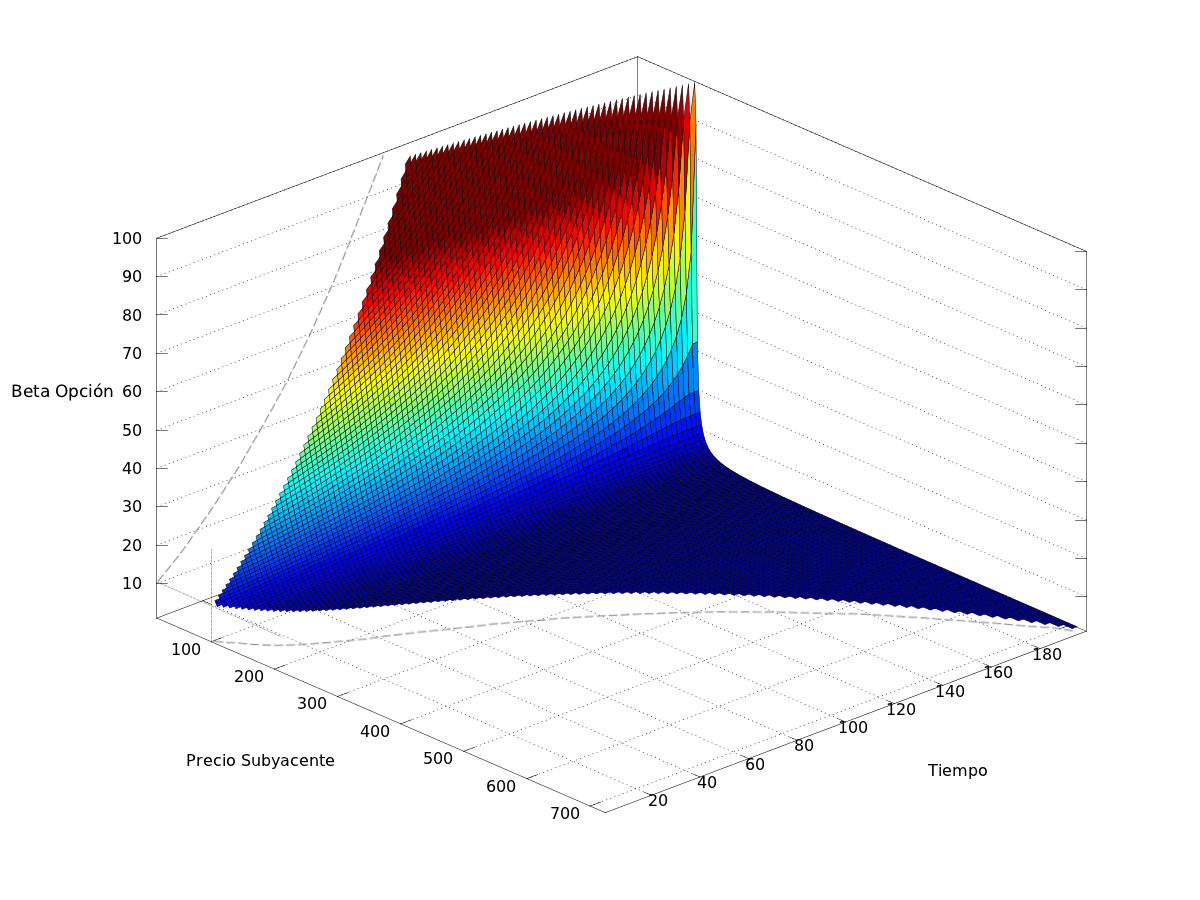
\includegraphics[width=1\textwidth]{Images/beta3d.png}
\caption{Evolución de la $\beta$ de la opción en el árbol binomial}
\label{fig:beta3d}
\end{figure}

Si se evalúa la evolución del \textit{beta} a lo largo del árbol para los mismos precios del subyacente, se puede observar que esta crece a medida que el plazo a la fecha de ejercicio disminuye. Sin embargo, la relación no es lineal. El crecimiento del \textit{beta} es bajo cuando el plazo al vencimiento es alto y crece rápidamente en los últimos periodos. Esta medida de riesgo, en función del plazo al vencimiento evoluciona de forma exponencial decreciente, de forma que se asemeja a una función del tipo $\beta(T-t) \sim a/(T-t)^b$ donde $a$ y $b$ son parámetros a estimar en cada caso. Esta función no tiene por objetivo ser exacta, sino facilitar la comprensión.

En el caso de las opciones \textit{put} o de venta, el comportamiento del \textit{beta} es análogo y a la vez más complejo. Si se descompone el valor de la opción entre el valor que otorga esta como seguro y el tiempo del dinero, se puede ver que ambos factores afectan de forma contraria al precio. Por esta razón, existen casos en donde el \textit{put} puede tener un \textit{beta} menor a la del activo subyacente \cite{optionsmarkets}.


\section{Más \textit{beta}: Casos particulares}

Existen dos casos particulares en donde el \textit{beta} exhibe valores distintos a los explicados anteriormente. 

Primero, en los nodos del último paso del árbol el \textit{beta} de la opción esta indefinida. Esto se debe a que no tiene sentido hablar de CAPM en un punto especifico ya que los rendimientos y por lo tanto el tiempo son cruciales en este modelo. Dada la definición matemática $\beta_f = Cov(r_f; r_M) / \Sigma_M^2$, la rentabilidad del activo es un parámetro tiempo-dependiente, por lo que la beta puntual no se encuentra definida.

Segundo, existe un área triangular en los últimos nodos del árbol cuando la opción se encuentra \textit{out-of-the-money} en donde el \textit{beta} está también indefinida. La figura \ref{fig:betaarbolchico} muestra este comportamiento. La inexistencia de un valor para el \textit{beta} surge del hecho de que no existe ningún camino posible que conduzca a la opción a estar \textit{in-the-money}. Si la opción vale en esos casos por definición cero ($Cov(r_f; r_M)$), la réplica es posible aunque innecesaria, por lo que el \textit{beta} del activo será indefinida. A medida que se incrementa la cantidad de pasos este error tiende a reducirse aunque nunca se elimina por completo en un árbol binomial.

Como se mencionó anteriormente, estos dos problemas tienden a desaparecer a medida que se incrementa la cantidad de pasos que se utiliza en el árbol binomial, por lo que no invalida el modelo. El segundo problema mencionado es sin duda una de las fuentes de error ya que esto no ocurre en modelos en tiempo continuo.







\chapter{Conclusión}\label{Conclusion}

En los primeros capítulos se detalla las caracteristicas de los principales modelos para valuar acciones y opciones. El \textit{Capital Asset Pricing Model} se desarrolla en base a un supuesto de equilibrio de mercado, en donde todos los inversores comparten expectativas homogeneas y optimizan su portafolio eficientemente en función de estas. Por el otro lado, existen modelos de valuación de opciones que se basan en la idea de que no existen oportunidades de arbitraje. Este supuesto mucho más fuerte es independiente de las expectativas de los inversores y por ende cualquiera debería realizar la misma valuación.

A lo largo del último capitulo se exploró la capacidad de valuación de opciones utilizando el primer modelo analizado. El primer resultado fue que CAPM es matemáticamente compatible con el modelo de Black-Scholes, es decir que realizando un portafolio replicante y valuandolo con CAPM conduce a la misma ecuación diferencial que esté último. Es este caso, la derivación de la ecuación diferencial de Black-Scholes es dependiente de CAPM, lo que sustenta la validez de la valuación mediante B\&S en el equilibrio general.

La valuación a modo de ejemplo de una opción permitio verificar lo esperable (dada la equivalencia matemática), ambos modelos otorgan iguales resultados en la valuación de estos instrumentos. El problema de CAPM se presenta en términos prácticos, no teóricos, cuando para alcanzar una valuación precisa de una opción es necesaria la construcción de árbol con una enorme cantidad de nodos. Esto conlleva una gran cantidad de cálculos y de recursos necesarios que hacen que este proceso sea considerablemente lento e ineficiente.

El \textit{beta} de las opciones en términos teóricos es siempre mayor que la de la acción subyacente para el caso de los \textit{calls} y en general mayor para los \textit{puts}. Esto se debe a que las opciones pueden ser entendidas como una compra apalancada del subyacente. Las pruebas que se realizaron mostraron que una opción \textit{at-the-money} puede tener un \textit{beta} 10 o 20 veces superior a la del subyacente fácilmente. Si bien esto no es una regla aplicable a todas las opciones, se puede observar la magnitud del riesgo que estas presentan.

Por último, la evolución del \textit{beta} de la opción en funcion del tiempo y del precio del subyacente presenta un comportamiento exponencial cuando la opción se torna más \textit{out-of-the-money}, o se reduce el tiempo al vencimiento. Es por eso que las opciones \textit{out-of-the-money} y con un reducido tiempo al vencimiento presentan un riesgo decenas de veces mayor al del activo subyacente; por el otro lado, las opciones con características opuestas presentan un riesgo bajo aunque en general (según se trate de opciones de compra o venta) mayor al del subyacente.






\addcontentsline{toc}{part}{Anexos}
\appendix

\chapter{Código fuente árbol binomial con CAPM}\label{anexocodigoapp}
% \addcontentsline{toc}{chapter}{Anexo I: Código fuente de la aplicación}


En la figura \eqref{CodigoApp} se presenta el código fuente del programa desarrollado para evaluar el árbol binomial mediante CAPM.
El mismo fue desarrollado en C\#.NET y puede ser compilado usando el \textit{SDK} de \textit{.NET} o de \textit{Mono}. El código para evaluar multiples veces el árbol y generar los gráficos incluidos en este trabajo se omite por razones de simplicidad.

% http://texblog.wordpress.com/2008/04/02/include-source-code-in-latex-with-listings/

\lstset{numbers=left, stepnumber=1, basicstyle=\footnotesize, frame=single, language=C++, 
	breaklines=true, breakatwhitespace=true, tabsize=2, showstringspaces=false,
	caption=Código fuente para el cálculo de un árbol binomial utilizando CAPM.,
	label=CodigoApp}

\begin{lstlisting}
using System;
using System.Collections.Generic;
using System.Runtime.CompilerServices;
	
public class Node
{
	public int NodeIndex { get; set; }
	public int StepNumber { get; set; }
	
	public decimal StockPrice { get; set; }
	public decimal OptionPrice { get; set; }
}

public abstract class BinTree
{
	private List<Node> nodeList;
	public int NumberOfSteps { get; set; }
	private int NodeCount { get; set; }
	
	// Tree Properties
	public decimal Volatility { get; set; }
	public decimal InitialStockPrice { get; set; }
	public decimal StrikePrice { get; set; }
	public decimal TotalTimeYears { get; set; }
	public decimal RiskFree { get; set; }
	public decimal MarketRiskPremium { get; set; }
	public decimal StockBeta { get; set; }
	
	private decimal? deltaT;
	public decimal DeltaT
	{
		get{
			if (deltaT == null)
				deltaT = TotalTimeYears / NumberOfSteps;
			return deltaT.Value;
		}
	}
	
	private decimal? mu;
	public decimal Mu
	{
		get{
			if (mu == null) 
				mu = (decimal)Math.Exp((double)Volatility * Math.Sqrt((double)DeltaT));
			return mu.Value;
		}
	}
	
	private decimal? de;
	public decimal De
	{
		get{
			if (de == null) de = 1/mu;
			return de.Value;
		}
	}

	// Constructor
	public BinTree (int numberOfSteps) {
		if (numberOfSteps < 2)
			throw new ArgumentException("Number of steps must be 2 or greater.", "numberOfSteps");
	
		NumberOfSteps = numberOfSteps;
		nodeList = new List<Node>(CalculateTotalNodes(numberOfSteps));
		
		BuildTree();
	}
	
	private void BuildTree() {
		for (int step = 1; step <= NumberOfSteps; step++) {
			
			int firstNode = CalculateTotalNodes(step-1)+1;
			int lastNode = CalculateTotalNodes(step);
			for (int idx = firstNode; idx <= lastNode; idx++) {
				
				var node = new Node();
				node.StepNumber = step;
				node.NodeIndex = idx;
				nodeList.Add(node);
				
				if (idx != nodeList.Count)
					throw new Exception("Node was added to the wrong possition");
			}
		}
    		NodeCount = nodeList.Count;
	}
	
	public void CalculateStockPrices() {
		var rootNode = GetRootNode();
		rootNode.StockPrice = InitialStockPrice;

		for (int step = 2; step <= NumberOfSteps; step++) {
			bool isFirstNodeInStep = true;
			foreach (var node in IterateNodesOfStep(step)) {
				if (isFirstNodeInStep) {
					// If it's the first node, the value is S*u
					isFirstNodeInStep = false;

					if (step == 2) {
						node.StockPrice = rootNode.StockPrice * Mu;
					} else {
						var downParentNode = CalculateTotalNodes(step-2)+1;
						node.StockPrice = nodeList[downParentNode-1].StockPrice * Mu;
					}
				} else {
					// Nodes other than the first one can be calculated as S*d
					int nodeOffset = CalculateTotalNodes(step) - node.NodeIndex;
					int upParentNode = CalculateTotalNodes(step - 1) - nodeOffset;
					node.StockPrice = nodeList[upParentNode-1].StockPrice * De;
				}
			}
		}
	}
	
	public abstract void CalculateOptionPrices();
	
	// Static Index Based Helper Methods
	public static int CalculateTotalNodes(int numberOfSteps) {
		if (numberOfSteps <= 0) return 0;
		return (numberOfSteps + 1) * numberOfSteps / 2;
	}
	
	public static int GetIndexFirstNodeInStep(int stepNumber) {
		return CalculateTotalNodes(stepNumber-1) + 1;
	}
	
	public static int GetIndexLastNodeInStep(int stepNumber) {
		return CalculateTotalNodes(stepNumber);
	}
	
	public Node GetRootNode() {
		return nodeList[0];
	}
	
	public Node GetFirstNodeInStep(int stepNumber) {
		if (stepNumber > NumberOfSteps) return null;
		return nodeList[GetIndexFirstNodeInStep(stepNumber)-1];
	}
	
	public Node GetLastNodeInStep(int stepNumber) {
		if (stepNumber > NumberOfSteps) return null;
		return nodeList[GetIndexLastNodeInStep(stepNumber)-1];
	}
	
	public int GetStepFromNode(Node node) {
		return node.StepNumber;
	}
	
	public Node GetUpDependantNode(Node node) {
		int idx = node.NodeIndex + CalculateTotalNodes(node.StepNumber) - CalculateTotalNodes(node.StepNumber - 1);
		if (NodeCount < idx) return null;
			return nodeList[idx-1];
	}
	
	public Node GetDownDependantNode(Node node) {
		int idx = node.NodeIndex + CalculateTotalNodes(node.StepNumber) - CalculateTotalNodes(node.StepNumber - 1) + 1;
		if (NodeCount < idx) return null;
			return nodeList[idx-1];
	}
	
	public IEnumerable<Node> IterateNodesOfStep(int stepNumber) {
		int firstNode = CalculateTotalNodes(stepNumber-1)+1;
		int lastNode = CalculateTotalNodes(stepNumber);
		for (int idx = firstNode; idx <= lastNode; idx++)
			yield return nodeList[idx-1];
	}
}

public class CapmBinTree : BinTree
{
	public CapmBinTree (int numberOfSteps) : base(numberOfSteps) {}
	
	public override void CalculateOptionPrices() {
		// First, calculate last step prices
		foreach (var node in IterateNodesOfStep(NumberOfSteps)) {
			node.OptionPrice = Math.Max(node.StockPrice - StrikePrice, 0);
		}

		decimal rfTimesDelta = (decimal)Math.Exp((double)RiskFree * (double)DeltaT);
		
		// Now, in previous steps... 
		for (int step = NumberOfSteps-1; step >= 1; step--) {
			// calculate the beta and then the option price
			foreach (var node in IterateNodesOfStep(step)) {
				CalcOptionPrice(node, rfTimesDelta, step);
			}
		}
	}

	private void CalcOptionPrice(Node node, decimal rfTimesDelta, int step) {
		decimal rfTimesDelta = (decimal)Math.Exp((double)RiskFree * (double)DeltaT);

		var upDep = GetUpDependantNode(node);
		var downDep = GetDownDependantNode(node);
		
		// Delta OK!
		 decimal delta = (upDep.OptionPrice - downDep.OptionPrice) /
            			(upDep.StockPrice - downDep.StockPrice);
		
		// Bond OK!
		decimal bond = (Mu * downDep.OptionPrice - De * upDep.OptionPrice) /
      			      ((Mu - De) * rfTimesDelta);
		
		decimal totalReplPortfolio = (delta * node.StockPrice + bond);
		decimal optionBeta = 0;
		if (totalReplPortfolio != 0)
	                optionBeta = delta * node.StockPrice / totalReplPortfolio * StockBeta;

		decimal rc = RiskFree + optionBeta * MarketRiskPremium;
		decimal rs = RiskFree + StockBeta * MarketRiskPremium;
		decimal p = (rs * DeltaT - De + 1) / (Mu - De);

		node.OptionPrice = (p * upDep.OptionPrice + (1 - p) * downDep.OptionPrice) / 
			(1 + rc * DeltaT);
	}
}
\end{lstlisting}


\chapter{Herramientas matemáticas}\label{anexoherramientasbs}

\section*{Lema de Ito}

Para averiguar $ \tilde{S}(T) $ hay que resolver la ecuación diferencial, lo cual se resuelve es resulto por el Lema de Ito. El mismo sirve para resolver ecuaciones diferenciales estocásticas, que son diferenciables de segundo orden.

Aplicando el teorema de Taylor para la función logarítmica $ f(S) $, donde $ S $ sigue un movimiento browniano geométrico:

\begin{align}
	f(S) &= ln(S) \label{defF}\\
	dS &= \mu S dt + \sigma S dW \label{ecuacionDiferencialS}
\end{align}

Y por el lema de Ito, obtenemos:

\begin{equation}
	df = \frac{\partial f}{\partial S} dS + 
		\frac{\partial f}{\partial t} dt + 
		\frac{1}{2} \frac{\partial^2 f}{\partial S^2} (dS)^2 \label{ito-ftaylor}
\end{equation}

con $ \frac{\partial f}{\partial S} = \frac{1}{S} $ y $ \frac{\partial^2 f}{\partial S^2} = -\frac{1}{S^2} $. En la expansión de Taylor se consideran despreciables los términos de grado mayor a dos.

Reemplazando $ dS $ y las derivadas parciales en la ecuación \eqref{ito-ftaylor} se llega a que:

\[ df = (\mu - \frac{\sigma^2}{2}) dt + \sigma dW \]

Por último reemplazamos $ f $ por su definición \eqref{defF} y obtenemos:

\begin{equation}
	d \log{S} = (\mu - \frac{\sigma^2}{2}) dt + \sigma dW \label{ito-eqdiferencial}
\end{equation}


Ahora, para calcular $S(T)$ debemos resolver la ecuación diferencial \eqref{ito-eqdiferencial}. Integrando a ambos lados de la ecuación entre 0 y $ t $:

\begin{equation}
	\int_0^t \,\mathrm{d}\log S = 
		\int_0^t \left(\mu - \frac{\sigma^2}{2}\right) \,\mathrm{d}t +
		\int_0^t \sigma \,\mathrm{d}W \label{ito-integraldefinida}
\end{equation}

Ahora, si resolvemos las integrales directas y aplicando el teorema de Newton-Leibniz, veremos que del último término surge $ W_0 $. Como $ \sigma W_0 $ es una variable aleatoria en el momento cero, se puede omitir ya que el término estocastico en el momento inicial podría considerarse nulo; de otra forma, cualquier variación puede considerarse incluida en el término deterministico. $ W_0 $ puede ser reemplazado por su definición \eqref{ito-dw}, de forma que la ecuación \eqref{ito-integraldefinida} se convierte en:

\begin{equation}
	\log \tilde{S}(T) - \log S(0) = 
		\left(\mu - \frac{\sigma^2}{2}\right) T +
		\sigma \sqrt{T} Z
\end{equation}

Dado que $ Z $ es una variable aleatoria con distribución normal estandar, se puede ver que:

\begin{subequations}
\begin{align}
	\log \left( \frac{\tilde{S}(T)}{S(0)} \right) &= N\left[
		\left(\mu - \frac{\sigma^2}{2}\right) T;
		\sigma^2 T
		\right] \label{distribucionRendimiento}\\
	\log \tilde{S}(T) &= N\left[
		\log S(0) + \left(\mu - \frac{\sigma^2}{2}\right) T;
		\sigma^2 T
		\right] \label{distribucionPrecio}
\end{align}
\end{subequations}

En \eqref{distribucionRendimiento} se puede ver que la rentabilidad en tiempo continuo sigue una distribución normal. El precio del subyacente, en cambio, tiene una distribución log-normal, razon por la cual el precio nunca puede ser menor a cero. Si la distribución del precio fuese normal, podría ocurrir que el precio en algún momento tomase un valor negativo, lo cual sería incorrecto.

Por último, aplicando el operador $e$ en ambos lados de la ecuación \eqref{distribucionRendimiento}, y reacomodando llegamos a la formula final que muestra el valor del subyacente al final del periodo $T$:

\begin{equation}
	S_T = S_0 e^{\left(\mu-\frac{\sigma^2}{2}\right)T+\sigma \sqrt{T} Z} \label{formulaST-desde0}
\end{equation}

Considerando que esta formula es valida para cualquier momento durante la existencia de la opción, podríamos extender la fórmula para cualquier momento $0 \leq t \leq T$. Llamamos $\tau$ al tiempo de vida remanente de la opción, por lo que $\tau=T-t$. Entonces, generalizando la ecuación \eqref{formulaST-desde0}, obtenemos:

\begin{equation}
	S_T = S_t e^{\left(\mu-\frac{\sigma^2}{2}\right)\tau+\sigma \sqrt{\tau} Z} \nonumber
\end{equation}



\chapter{Gráficos arboles binomiales}\label{anexograficos}

A continuación se incluyen diversos gráficos correspondientes al mismo árbol binomial de 10 pasos. Estos permiten observar la evolución de diferentes propiedades tales como la beta de la opción, el delta ($\Delta$) y el apalancamiento.

Los gráficos fueron realizados para una opción de compra con: precio inicial del subyacente = 100, precio de ejercicio = 105, tiempo = 1/2 año, volatilidad = 20\%, tasa libre de riesgo = 3\%, prima de riesgo del mercado ($\overline{r_M} - r_f$) es del 6\% y $\beta_S$ = 1.

\begin{figure}[H]
\centering
\includegraphics[width=1\textwidth]{Images/tree-betas.jpg}
\caption{Evolución de la $\beta$ de una opción en el árbol binomial de 10 pasos}
\label{fig:betaarbolchico}
\end{figure}

En la figura \ref{fig:deltaarbolchico} se ve la evolución del $\Delta$ (en rojo) con el cual se puede replicar una opción en un árbol binomial de 10 pasos. También se observa en azul el nivel de apalancamiento necesario para replicarla.

\begin{figure}[H]
\centering
\includegraphics[width=1\textwidth]{Images/tree-delta-leverage.jpg}
\caption{Evolución del $\Delta$ y el apalancamiento en un árbol binomial de 10 pasos.}
\label{fig:deltaarbolchico}
\end{figure}



\input{Referencias}

\end{document}
